\section{Deep Learning\label{sec:DL}}
%%%%%%%%%%%%%%%%%%%%%%%%%%%%%%%%%%%%%%%%%%%%%%%%%%%%%%%%%%%%%%%%%%%%%%%%%%%%%%%%
\Gls{DL} is a field of \gls{ML} that is primarily concerned with the learning of
representations of data. At the core of \gls{DL} is the use of \glspl{MLP}, used
to model these representations. \Glspl{MLP} are fully connected layers of
biologically inspired artifical neurons, also known as \textbf{perceptrons}. A
brief history are these biologically inspired models are covered in
\autoref{ssec:perceptrons} with adapted notation from the field of \gls{DL}.
Although not all practices in \gls{DL}, strictly speaking, make use of
\glspl{MLP}, they are a fundamental concept which must be understood in the
stepping stones towards concepts of higher complexity in the field.
\autoref{ssec:mlps} covers this concept, extending directly on their composite
component: perceptrons.

\Glspl{MLP} are also called \textbf{feedfoward} as information is propagated in
only a forward direction, as apposed to exhibiting \textbf{feedback} connections,
where intermediate computations are fed back into the network. When feedforward
networks are extended to include feedback connections, they are called
\textbf{\glspl{RNN}}. These types of networks excel at learning temporal
features, exhibiting a refined hypothesis space favouring sequenced information,
such as a series of chronological observations. \autoref{ssec:rnn} covers this
type of \gls{DNN}, and the prominent sub-type of \glspl{RNN}: \glspl{LSTM}.

One category of neural networks which are similar to \glspl{MLP}, popular in
contemporary research, are \glspl{CNN}. These \glspl{DNN} are essentially
\glspl{MLP} which omit the property of being fully connected, in favour of
refining the hypothesis space towards detection of spatially-related features.

The main difference between a \gls{NN} and a
traditional \gls{ML} algorithm is that the neural network is a function of the
data, rather than the data itself.

\subsection{Brief History of the Perceptron\label{ssec:perceptrons}}
%%%%%%%%%%%%%%%%%%%%%%%%%%%%%%%%%%%%%%%%%%%%%%%%%%%%%%%%%%%%%%%%%%%%%%%%%%%%%%%%

The McCullock-Pitts neuron, an earlier iteration of an artificial neuron, was
proposed by McCulloch and Pitts in the field of neuroscience in 1943
\cite{McCulloch1943}. Their work contended that neurons with a binary activation
function were analogous to first order logic sentences. The perception of
artifical neurons changed with Hebb's work in 1949, where he proposed an idea
which has come to be known as Hebb's rule:

\begin{fancyquotes}
    Let us assume that the persistence or repetition of a reverberatory activity
    (or ``trace") tends to induce lasting cellular changes that add to its
    stability. [...] When an axon of cell A is near enough to excite a cell B
    and repeatedly or persistently takes part in firing it, some growth process
    or metabolic change takes place in one or both cells such that A’s
    efficiency, as one of the cells firing B, is increased. \cite{10.1007/978-3-642-70911-1_15}
\end{fancyquotes}

This theory is often summaraized as \textit{``Cells that fires together, wire
together"} \cite{doi:10.1126/science.7912852}, which persists today in the
gradient-based learning at the core of contemporary \gls{DL}. The perceptron was
proposed by Rosenblatt \cite{Rosenblatt_1957_6098} in his technical report
funded by the United States Office of Naval Research
\cite{doi:10.1177/030631296026003005} in 1957. Rosenblatt incorporated Hebb's
findings into the McCullock-Pitts neuron.

The \textit{perceptron} is arguably the most fundamental concept in deep
learning, describing a mathematical model of a biological neuron. There are two
different sets of notation which exist when dealing with the bias of a
perceptron. One involves the inclusion of a unit constant in the input vector
$\mathbf{x}$, with the bias being specified by the value of the first weight
$w_0$. An alternative notation exists which treats the bias as a standalone
value $b$. The latter notation will be used, as it is the preferred notation in
contemporary deep learning research. The notation defining the mapping of a
perceptron is then: $f(\gls{ml:x};\gls{w_vec},
\gls{b})=\gls{ml:x}^T\gls{w_vec}+\gls{b}$;
$\gls{ml:x}\in\gls{set:R}^{\gls{ml:n_x}}$,
$\gls{w_vec}\in\gls{set:R}^{\gls{ml:n_x}}$, $\gls{b}\in\gls{set:R}$. Furthermore
the model parameters, \gls{ml:theta}, as introduced in
\autoref{sec:capoverunder}, are defined by the union of the bias and weight
vectors: $\gls{ml:theta}=\{\gls{w_vec},\gls{b}\}$.
\begin{figure}[htbp]
    \centering
    % MIT License
%
% Copyright (c) 2021 Geoffrey H. Garrett
%
% Permission is hereby granted, free of charge, to any person obtaining a copy
% of this software and associated documentation files (the "Software"), to deal
% in the Software without restriction, including without limitation the rights
% to use, copy, modify, merge, publish, distribute, sublicense, and/or sell
% copies of the Software, and to permit persons to whom the Software is
% furnished to do so, subject to the following conditions:
%
% The above copyright notice and this permission notice shall be included in all
% copies or substantial portions of the Software.
%
% THE SOFTWARE IS PROVIDED "AS IS", WITHOUT WARRANTY OF ANY KIND, EXPRESS OR
% IMPLIED, INCLUDING BUT NOT LIMITED TO THE WARRANTIES OF MERCHANTABILITY,
% FITNESS FOR A PARTICULAR PURPOSE AND NONINFRINGEMENT. IN NO EVENT SHALL THE
% AUTHORS OR COPYRIGHT HOLDERS BE LIABLE FOR ANY CLAIM, DAMAGES OR OTHER
% LIABILITY, WHETHER IN AN ACTION OF CONTRACT, TORT OR OTHERWISE, ARISING FROM,
% OUT OF OR IN CONNECTION WITH THE SOFTWARE OR THE USE OR OTHER DEALINGS IN THE
% SOFTWARE.

%%%%%%%%%%%%%%%%%%%%%%%%%%%%%%%%%%%%%%%%%%%%%%%%%%%%%%%%%%%%%%%%%%%%%%%%%%%%%%%
% ACKNOWLEDGEMENTS
%%%%%%%%%%%%%%%%%%%%%%%%%%%%%%%%%%%%%%%%%%%%%%%%%%%%%%%%%%%%%%%%%%%%%%%%%%%%%%%
% Design and implementation of this diagram was inspired and adapted from:
% https://tex.stackexchange.com/questions/104334/tikz-diagram-of-a-perceptron

%%%%%%%%%%%%%%%%%%%%%%%%%%%%%%%%%%%%%%%%%%%%%%%%%%%%%%%%%%%%%%%%%%%%%%%%%%%%%%%
% DEPENDENCIES
%%%%%%%%%%%%%%%%%%%%%%%%%%%%%%%%%%%%%%%%%%%%%%%%%%%%%%%%%%%%%%%%%%%%%%%%%%%%%%%
%\usepackage{tikz}
%\usetikzlibrary{decorations.pathreplacing}    % for TikZ braces
%\usetikzlibrary{positioning}                  % for TikZ relative positioning

%%%%%%%%%%%%%%%%%%%%%%%%%%%%%%%%%%%%%%%%%%%%%%%%%%%%%%%%%%%%%%%%%%%%%%%%%%%%%%%
% USER STYLING
%%%%%%%%%%%%%%%%%%%%%%%%%%%%%%%%%%%%%%%%%%%%%%%%%%%%%%%%%%%%%%%%%%%%%%%%%%%%%%%

% TikZ node design.
\tikzset{basic/.style={draw,text width=1em,text badly centered}}
\tikzset{input/.style={}}
\tikzset{output/.style={}}
\tikzset{weight/.style={basic,circle}}
\tikzset{hidden/.style={basic,circle}}
\tikzset{function/.style={basic,circle}}
\def\layersep{3em}
\def\transferx{9em}
\def\hiddenx{7em}
\def\hiddenxn{12em}

% Labels and symbols.
\def\activationlabel{activation function}  % activation function label
\def\activationsymbol{$\phi$}              % activation function symbol
\def\transferlabel{transfer function}      % transfer function label
\def\transfersymbol{$\sum$}                % transfer function symbol
\def\outputsymbol{$y$}                     % output symbol
\def\inputsymbol{$x$}                      % input symbol
\def\inputvecsymbol{$\mathbf{x}$}          % input vector symbol
\def\weightslabel{weights}                 % input vector symbol
\def\biassymbol{$b$}                       % bias symbol

\def\sep{4em}
\def\L{\gls{L}}       % number of hidden layers
\def\y{\gls{y_true}}  % output vector
\def\x{\gls{ml:x}}    % input vector
\def\h{\gls{a_vec}}   % hidden output
\def\nx{\gls{np:dim}[_\gls{fn:in}]}   % hidden output
\def\ny{\gls{np:dim}[_\gls{fn:out}]}   % hidden output
\def\a{\gls{dl:a}}   % hidden output
\def\z{\gls{dl:z}}   % hidden output

%%%%%%%%%%%%%%%%%%%%%%%%%%%%%%%%%%%%%%%%%%%%%%%%%%%%%%%%%%%%%%%%%%%%%%%%%%%%%%%
% TIKZ PICTURE
%%%%%%%%%%%%%%%%%%%%%%%%%%%%%%%%%%%%%%%%%%%%%%%%%%%%%%%%%%%%%%%%%%%%%%%%%%%%%%%
\begin{tikzpicture}

    \node[function] at ({\transferx}, -{int(2)})  (transfer) {\transfersymbol};
    \node[function, right=3em of transfer] (activation) {\activationsymbol};
    \node[below of=activation,font=\scriptsize,text width=3em] {\activationlabel};
    \node[below of=transfer,font=\scriptsize,text width=3em] {\transferlabel};
    \node[output, right=\layersep of activation] (output) {\outputsymbol};
    \path[draw,->] (transfer) -- node[above] {\z} (activation);
    \path[draw,->] (activation) -- node[above] {\a} (output);
%    \path[draw,->] (activation)(output);

    % Iterate through each row of units.
    \foreach \n [evaluate=\n as \p using {int(\n-1)}] in {0,1,2,3,4} {
        \ifnum \n=0
            \node[input] at (0, -\n) (X-\n) {$1$};
            \node[weight] at (\layersep, -\n) (W-\n) {$w_\n$};
        \else \ifnum \n=3
            \node[] at (0, -\n) (X-\n) {$\vdots$};
            \node[] at (\layersep, -\n) (W-\n) {$\vdots$};
        \else \ifnum \n=4
            \node[input] at (0, -\n) (X-\n) {$x_{\nx}$};
            \node[weight,label={[xshift=-0.0em]center:$w_{\nx}$}] at (\layersep, -\n) (W-\n) {\phantom{$w_{\nx}$}};
        \else
            \node[input] at (0, -\n) (X-\n) {$x_\n$};
            \node[weight] at (\layersep, -\n) (W-\n) {$w_\n$};
        \fi
        \fi
        \fi

        % Arrow from input to weight.
        \ifnum \n=3
        \else
            \path[draw,->] (X-\n) -- (W-\n);
                        \path[draw,->] (W-\n) -- (transfer);
        \fi

    }

    % Brace for bias.
    \node[left=1em of X-0] (bias-brace) {};
    \node[above=1em of bias-brace] (bias-brace-up) {};
    \node[below=1em of bias-brace] (bias-brace-down) {};
    \draw[decorate,decoration = {brace}] (bias-brace-down) --  (bias-brace-up);
    \node[left of=bias-brace,font=\scriptsize] {bias, \biassymbol};

    % Brace for input.
    \node[below=10em of bias-brace-down] (input-brace-down) {};
    \node[below=5em of bias-brace-down] (input-brace) {};
    \draw[decorate,decoration = {brace}] (input-brace-down) --  (bias-brace-down);
    \node[left of=input-brace,font=\scriptsize] {inputs, \inputvecsymbol};

    % Weights label.
    \node[below of=W-4,font=\scriptsize] {\weightslabel};

\end{tikzpicture}

    \captionsetup{format=hang} % hanging captions
    \caption{
        \textbf{Generalized illustration of a perceptron.} The mapping is
        defined by $f(\gls{ml:x};\gls{w_vec},
        \gls{b})=\gls{ml:x}^T\gls{w_vec}+\gls{b}$ where
        $\{\gls{w_vec},\gls{b}\}=\gls{ml:theta}$. The original formulation of
        the perceptron \cite{Rosenblatt_1957_6098} was intended to output a
        binary value, using a threshold step function, for classification
        purposes. The actual activation function \gls{dl:activation} has been
        generalized in order to relate the concept to modern deep learning
        techniques.
    }
    \label{fig:perceptron}
\end{figure}

\begin{equation}
    a=g\bigg(\sum_{k=0}^{\gls{ml:n_x}}{w_k}x_k + b\bigg)=g(z)
\end{equation}


%Rosenblatt's incorporated the model of  Rosenblatt
%incorporated the findings of Hebb \cite{10.1007/978-3-642-70911-1_15} into the
%model proposed by A set of inputs \gls{ml:x} would be weighted before being
%passed through a threshold step activation function \gls{dl:activation}.
%\autoref{fig:perceptron} shows a more general formulation which applies to the
%field of deep learning, with any activation function, \gls{dl:activation},
%mimicking a level of excitation akin to a biological neuron in response to its
%stimulus \gls{ml:x}.

\begin{figure}[!htp]
    \centering
    \begin{subfigure}[b]{0.70\textwidth}
        \centering
        % MIT License
%
% Copyright (c) 2021 Geoffrey H. Garrett
%
% Permission is hereby granted, free of charge, to any person obtaining a copy
% of this software and associated documentation files (the "Software"), to deal
% in the Software without restriction, including without limitation the rights
% to use, copy, modify, merge, publish, distribute, sublicense, and/or sell
% copies of the Software, and to permit persons to whom the Software is
% furnished to do so, subject to the following conditions:
%
% The above copyright notice and this permission notice shall be included in all
% copies or substantial portions of the Software.
%
% THE SOFTWARE IS PROVIDED "AS IS", WITHOUT WARRANTY OF ANY KIND, EXPRESS OR
% IMPLIED, INCLUDING BUT NOT LIMITED TO THE WARRANTIES OF MERCHANTABILITY,
% FITNESS FOR A PARTICULAR PURPOSE AND NONINFRINGEMENT. IN NO EVENT SHALL THE
% AUTHORS OR COPYRIGHT HOLDERS BE LIABLE FOR ANY CLAIM, DAMAGES OR OTHER
% LIABILITY, WHETHER IN AN ACTION OF CONTRACT, TORT OR OTHERWISE, ARISING FROM,
% OUT OF OR IN CONNECTION WITH THE SOFTWARE OR THE USE OR OTHER DEALINGS IN THE
% SOFTWARE.

%%%%%%%%%%%%%%%%%%%%%%%%%%%%%%%%%%%%%%%%%%%%%%%%%%%%%%%%%%%%%%%%%%%%%%%%%%%%%%%
% ACKNOWLEDGEMENTS
%%%%%%%%%%%%%%%%%%%%%%%%%%%%%%%%%%%%%%%%%%%%%%%%%%%%%%%%%%%%%%%%%%%%%%%%%%%%%%%
% Design and implementation of this diagram was inspired and adapted from:
% https://tex.stackexchange.com/questions/104334/tikz-diagram-of-a-perceptron

%%%%%%%%%%%%%%%%%%%%%%%%%%%%%%%%%%%%%%%%%%%%%%%%%%%%%%%%%%%%%%%%%%%%%%%%%%%%%%%
% DEPENDENCIES
%%%%%%%%%%%%%%%%%%%%%%%%%%%%%%%%%%%%%%%%%%%%%%%%%%%%%%%%%%%%%%%%%%%%%%%%%%%%%%%
%\usepackage{tikz}
%\usetikzlibrary{decorations.pathreplacing}    % for TikZ braces
%\usetikzlibrary{positioning}                  % for TikZ relative positioning

%%%%%%%%%%%%%%%%%%%%%%%%%%%%%%%%%%%%%%%%%%%%%%%%%%%%%%%%%%%%%%%%%%%%%%%%%%%%%%%
% USER STYLING
%%%%%%%%%%%%%%%%%%%%%%%%%%%%%%%%%%%%%%%%%%%%%%%%%%%%%%%%%%%%%%%%%%%%%%%%%%%%%%%

% TikZ node design.
\tikzset{basic/.style={draw,text width=1em,text badly centered}}
\tikzset{input/.style={}}
\tikzset{output/.style={}}
\tikzset{weight/.style={basic,circle}}
\tikzset{hidden/.style={basic,circle}}
\tikzset{function/.style={basic,circle}}
\def\layersep{3em}
\def\transferx{9em}
\def\hiddenx{7em}
\def\hiddenxn{12em}

% Labels and symbols.
\def\activationlabel{threshold step}  % activation function label
\def\activationsymbol{$H$}              % activation function symbol
\def\transferlabel{sum}      % transfer function label
\def\transfersymbol{$\sum$}                % transfer function symbol
\def\outputsymbol{$\text{AND}(x_1, x_2)$}                     % output symbol
\def\inputsymbol{$x$}                      % input symbol
\def\inputvecsymbol{$\mathbf{x}$}          % input vector symbol
\def\weightslabel{weights}                 % input vector symbol
\def\biassymbol{$b$}                       % bias symbol

\def\sep{4em}
\def\L{\gls{L}}       % number of hidden layers
\def\y{\gls{y_true}}  % output vector
\def\x{\gls{ml:x}}    % input vector
\def\h{\gls{a_vec}}   % hidden output
\def\nx{\gls{ml:n_x}}   % hidden output
\def\ny{\gls{ml:n_y}}   % hidden output
\def\z{\gls{dl:z}}   % hidden output
\def\a{\gls{dl:a}}   % hidden output

%%%%%%%%%%%%%%%%%%%%%%%%%%%%%%%%%%%%%%%%%%%%%%%%%%%%%%%%%%%%%%%%%%%%%%%%%%%%%%%
% TIKZ PICTURE
%%%%%%%%%%%%%%%%%%%%%%%%%%%%%%%%%%%%%%%%%%%%%%%%%%%%%%%%%%%%%%%%%%%%%%%%%%%%%%%
\begin{tikzpicture}

    \node[function] at ({\transferx}, -{int(2)})  (transfer) {\transfersymbol};
    \node[function, right=3em of transfer] (activation) {\activationsymbol};
    \node[below of=activation,font=\scriptsize,text width=3em] {\activationlabel};
    \node[below of=transfer,font=\scriptsize,text width=3em] {\transferlabel};
    \node[output, right=\layersep of activation] (output) {\outputsymbol};
    \path[draw,->] (transfer) -- node[above] {\z} (activation);
    \path[draw,->] (activation) -- node[above] {\a} (output);

    \node[input] at (0, -1) (X-1) {$1$};
    \def\wone{$-1$}
    \node[weight, label={[xshift=-0.0em]center:\wone}] at (\layersep, -1) (W-1) {\phantom{\wone}};

    \node[input] at (0, -2) (X-2) {$x_1$};
    \def\wtwo{$1$}
    \node[weight, label={[xshift=-0.0em]center:\wtwo}] at (\layersep, -2) (W-2) {\phantom{\wtwo}};

    \node[input] at (0, -3) (X-3) {$x_2$};
    \def\wthree{$1$}
    \node[weight, label={[xshift=-0.0em]center:\wthree}] at (\layersep, -3) (W-3) {\phantom{\wthree}};

    \path[draw,->] (X-1) -- (W-1);
    \path[draw,->] (X-2) -- (W-2);
    \path[draw,->] (X-3) -- (W-3);
    \path[draw,->] (W-1) -- (transfer);
    \path[draw,->] (W-2) -- (transfer);
    \path[draw,->] (W-3) -- (transfer);

    % Brace for bias.
    \node[left=1em of X-1] (bias-brace) {};
    \node[above=1em of bias-brace] (bias-brace-up) {};
    \node[below=1em of bias-brace] (bias-brace-down) {};
    \draw[decorate,decoration = {brace}] (bias-brace-down) --  (bias-brace-up);
    \node[left of=bias-brace,font=\scriptsize] {bias, \biassymbol};

    % Brace for input.
    \node[below=4.5em of bias-brace-down] (input-brace-down) {};
    \node[below=2.25em of bias-brace-down] (input-brace) {};
    \draw[decorate,decoration = {brace}] (input-brace-down) --  (bias-brace-down);
    \node[left of=input-brace,font=\scriptsize] {inputs, \inputvecsymbol};

    % Weights label.
    \node[below of=W-3,font=\scriptsize] {\weightslabel};

\end{tikzpicture}

        \captionsetup{format=hang} % hanging captions
        \subcaption{Perceptron mapping}
        \label{fig:perceptron:and:mapping}
    \end{subfigure}\hfil
    \begin{subfigure}[b]{0.29\textwidth}
        \centering
        \renewcommand{\arraystretch}{1.5}
        \begin{tabular}{C{0.1\linewidth}C{0.1\linewidth}|C{0.1\linewidth}}
            \hline
            $x_1$ & $x_2$ & $y$ \\ \hline
            0     & 0     & 0   \\
            0     & 1     & 0   \\
            1     & 0     & 0   \\
            1     & 1     & 1
        \end{tabular}
        \vspace{0.5cm}
        \subcaption{Truth table}
        \label{fig:perceptron:and:truth}
    \end{subfigure}\hfil
    \captionsetup{format=hang} % hanging captions
    \caption{
        \textbf{Truth table of the AND logic gate.}
    }
    \label{fig:perceptron:and}
\end{figure}



Rosenblatt's statements caused an unfortunate controversy in the fledgling field
of \gls{AI}. According to the New York Times, he reported the perceptron to be
\textit{``the embryo of an electronic computer that [the Navy] expects will be
able to walk, talk, see, write, reproduce itself and be conscious of its
existence."} \cite{Olazaran1996} The backlash from the \gls{AI} community

\subsubsection{Perceptrons and Logic Gates}




In its original form, the perceptron was used as a supervised learning method
for binary classifiers.

The primary criticism of the perceptron came in 1969 from Minsky and Papert
\cite{minsky69perceptrons}, where it was shown that the perceptron could only
solve \textit{linearly separable} functions, and failed to solve the XOR and
NXOR functions. They claimed that the work being done in this area was doomed to
failure due to these limitations, resulting in little subsequent research until
about the 1980's.


%
%\newpage
\newpage

\subsection{Multi-layer perceptrons\label{ssec:mlps}}
%%%%%%%%%%%%%%%%%%%%%%%%%%%%%%%%%%%%%%%%%%%%%%%%%%%%%%%%%%%%%%%%%%%%%%%%%%%%%%%%%
\Gls{MLPs}, otherwise known as \textbf{artificial neural networks} or
\textbf{feedforward neural networks}, are the fundamental models of \gls{DL}.
These models are biologically inspired, and make direct use of the concept of
the perceptron discussed in \autoref{ssec:perceptrons}. The primary extensions
involve the use of a variety of activation functions other than the threshold
step, and multiple layers of fully connected perceptrons, often referred to as
\textbf{neurons} or \textbf{units}. \gls{MLPs} are characterized as being
\textbf{fully-connected} which means that all the units in a layer are connected
to all units in the next. These models are often referred to as \textbf{deep
feedfoward networks} by virtue of having \textit{several} hidden layers. Note
that there is no universally accepted definition of what integer values of
perceptron layers \gls{dl:L} constitute deep and shallow networks, but generally
speaking: a shallow network will usually have one hidden layer and a deep
network will have several hidden layers. The mapping of an \gls{MLP} is defined
by $\gls{y_pred}=f(\gls{ml:x}; \gls{theta})$;
$\gls{ml:x}\in\gls{set:R}^{\gls{ml:n_x}}$;
$\gls{y_pred}\in\gls{set:R}^{\gls{ml:n_y}}$.

\begin{figure}[htp]
    \centering
    % MIT License
%
% Copyright (c) 2021 Geoffrey H. Garrett
%
% Permission is hereby granted, free of charge, to any person obtaining a copy
% of this software and associated documentation files (the "Software"), to deal
% in the Software without restriction, including without limitation the rights
% to use, copy, modify, merge, publish, distribute, sublicense, and/or sell
% copies of the Software, and to permit persons to whom the Software is
% furnished to do so, subject to the following conditions:
%
% The above copyright notice and this permission notice shall be included in all
% copies or substantial portions of the Software.
%
% THE SOFTWARE IS PROVIDED "AS IS", WITHOUT WARRANTY OF ANY KIND, EXPRESS OR
% IMPLIED, INCLUDING BUT NOT LIMITED TO THE WARRANTIES OF MERCHANTABILITY,
% FITNESS FOR A PARTICULAR PURPOSE AND NONINFRINGEMENT. IN NO EVENT SHALL THE
% AUTHORS OR COPYRIGHT HOLDERS BE LIABLE FOR ANY CLAIM, DAMAGES OR OTHER
% LIABILITY, WHETHER IN AN ACTION OF CONTRACT, TORT OR OTHERWISE, ARISING FROM,
% OUT OF OR IN CONNECTION WITH THE SOFTWARE OR THE USE OR OTHER DEALINGS IN THE
% SOFTWARE.

%%%%%%%%%%%%%%%%%%%%%%%%%%%%%%%%%%%%%%%%%%%%%%%%%%%%%%%%%%%%%%%%%%%%%%%%%%%%%%%
% ACKNOWLEDGEMENTS
%%%%%%%%%%%%%%%%%%%%%%%%%%%%%%%%%%%%%%%%%%%%%%%%%%%%%%%%%%%%%%%%%%%%%%%%%%%%%%%
% Adapted from:
% https://www.researchgate.net/figure/The-agent-environment-interaction-in-reinforcement-learning_fig1_328494763

%%%%%%%%%%%%%%%%%%%%%%%%%%%%%%%%%%%%%%%%%%%%%%%%%%%%%%%%%%%%%%%%%%%%%%%%%%%%%%%
% DEPENDENCIES
%%%%%%%%%%%%%%%%%%%%%%%%%%%%%%%%%%%%%%%%%%%%%%%%%%%%%%%%%%%%%%%%%%%%%%%%%%%%%%%
%\usepackage{tikz}
%\usetikzlibrary{decorations.pathreplacing}    % for TikZ braces
%\usetikzlibrary{positioning}                  % for TikZ relative positioning

%%%%%%%%%%%%%%%%%%%%%%%%%%%%%%%%%%%%%%%%%%%%%%%%%%%%%%%%%%%%%%%%%%%%%%%%%%%%%%%
% USER STYLING
%%%%%%%%%%%%%%%%%%%%%%%%%%%%%%%%%%%%%%%%%%%%%%%%%%%%%%%%%%%%%%%%%%%%%%%%%%%%%%%

% TikZ node design.
\tikzset{basic/.style={draw,text width=1em,text badly centered}}
\tikzset{input/.style={basic, fill=green!25, circle}}
\tikzset{output/.style={basic, fill=blue!25, circle}}
\tikzset{weight/.style={basic,circle}}
\tikzset{hidden/.style={basic,circle}}
\tikzset{function/.style={basic,circle}}
\def\layersep{3em}
\def\transferx{9em}
\def\hiddenx{7em}
\def\hiddenxn{12em}


\def\sep{4em}
\def\L{\gls{L}}       % number of hidden layers
\def\y{\gls{y_true}}  % output vector
\def\x{\gls{ml:x}}    % input vector
\def\h{\gls{a_vec}}   % hidden output
\def\nx{\gls{ml:n_x}}   % hidden output
\def\ny{\gls{ml:n_y}}   % hidden output


%%%%%%%%%%%%%%%%%%%%%%%%%%%%%%%%%%%%%%%%%%%%%%%%%%%%%%%%%%%%%%%%%%%%%%%%%%%%%%%
% TIKZ PICTURE
%%%%%%%%%%%%%%%%%%%%%%%%%%%%%%%%%%%%%%%%%%%%%%%%%%%%%%%%%%%%%%%%%%%%%%%%%%%%%%%
\begin{tikzpicture}
    \usetikzlibrary{decorations.pathreplacing}    % for TikZ braces
    \usetikzlibrary{positioning}                  % for TikZ relative positioning

    % input
    \foreach \n/\p in {0/1,1/2,2/3,3/4,4/5} {
        \ifnum \n=3
            % dots layer
            \node[] at (0, -\n) (X_\n) {$\vdots$};
            \node[] at (\hiddenx, -\n) (H1_\n) {$\vdots$};
            \node[right of=H1_\n] (M-\n) {$\ddots$};
            \node[below of=H1_2] (H2_\n) {$\vdots$};
            \node[below of=H2_2] (H2_\n) {$\vdots$};
            \node[right=5.7em of H2_\n] (Y_\n) {$\vdots$};
        \else
        \ifnum \n=4
            % n layer
            \node[input] at (0, -\n) (X_\n) {};
            \node[left of=X_\n] (I_\n) {$x_{\nx}$};
            \path[draw,->] (I_\n) -- (X_\n);
            \node[hidden] at (\hiddenx, -\n) (H1_\n) {}; %{$h_{n, 1}$};
            \node[right of= H1_\n] (M-\n) {$\ldots$};
            \node[hidden, right of= M-\n] (H2_\n) {}; % {$h_{n, m}$};
            \node[output, right= 5em of H2_\n] (Y_\n) {}; % {$h_{n, m}$};
            \node[right of=Y_\n] (O_\n) {$y_{\ny}$};
            \path[draw,->] (Y_\n) -- (O_\n);
        \else
            \node[input] at (0, -{\n}) (X_\n) {};
            \node[left of=X_\n] (I_\n) {$x_{\p}$};
            \path[draw,->] (I_\n) -- (X_\n);
            \node[hidden] at (\hiddenx, -\n) (H1_\n) {};%{$h_{\n, 1}$};
            \node[right of=H1_\n] (M-\n) {$\ldots$};
            \node[hidden, right of=M-\n] (H2_\n) {};% {$h_{\n, m}$};
            \node[output, right= 5em of H2_\n] (Y_\n) {}; % {$h_{n, m}$};
            \node[right of=Y_\n] (O_\n) {$y_\p$};
            \path[draw,->] (Y_\n) -- (O_\n);
        \fi
        \fi
    }

    % input layer connected to first hidden layer
    \foreach \j in {0,1,2,4} {
        \foreach \n in {0,1,2,4} {
            \path[draw,->] (X_\n) -- (H1_\j);
        }
    }

    % second hidden layer connected to output layer
    \foreach \j in {0,1,2,4} {
        \foreach \n in {0,1,2,4} {
            \path[draw,->] (H2_\n) -- (Y_\j);
        }
    }

    % labels
    \node[below of=X_4,font=\scriptsize, align=center] {input\\layer};
    \node[below of=Y_4,font=\scriptsize, align=center] {output\\layer};

    % brace for hidden layers
    \node[below=1em of M-4] (hidden-brace) {};
    \node[right=3em of hidden-brace] (hidden-brace-right) {};
    \node[left=3em of hidden-brace] (hidden-brace-left) {};
    \draw [decorate,decoration = {brace}] (hidden-brace-right) --  (hidden-brace-left);
    \node[below=0.5em of hidden-brace,font=\scriptsize] (hlayer) {hidden layer(s)};

\end{tikzpicture}


    \captionsetup{format=hang} % hanging captions
    \caption{
        \textbf{Generalized form of an \gls{MLP}}. Each layer, \textbf{excluding
        the input layer}, has associated weights, biases and activation
        functions. Furthermore, the layers are characterized as being
        \textbf{fully-connected}.
    }
    \label{fig:mlp}
\end{figure}

\autoref{fig:mlp} depicts the generalized concept of the \gls{MLP}. There are
three distinct types of layers: hidden, input, and output, for which
there is only one of each for the latter two. The input layer is simply the
input vector $\gls{ml:x}$, which does not have any weights, bias or activation
function associated to it.

\begin{figure}[htp]
    \centering
    % MIT License
%
% Copyright (c) 2021 Geoffrey H. Garrett
%
% Permission is hereby granted, free of charge, to any person obtaining a copy
% of this software and associated documentation files (the "Software"), to deal
% in the Software without restriction, including without limitation the rights
% to use, copy, modify, merge, publish, distribute, sublicense, and/or sell
% copies of the Software, and to permit persons to whom the Software is
% furnished to do so, subject to the following conditions:
%
% The above copyright notice and this permission notice shall be included in all
% copies or substantial portions of the Software.
%
% THE SOFTWARE IS PROVIDED "AS IS", WITHOUT WARRANTY OF ANY KIND, EXPRESS OR
% IMPLIED, INCLUDING BUT NOT LIMITED TO THE WARRANTIES OF MERCHANTABILITY,
% FITNESS FOR A PARTICULAR PURPOSE AND NONINFRINGEMENT. IN NO EVENT SHALL THE
% AUTHORS OR COPYRIGHT HOLDERS BE LIABLE FOR ANY CLAIM, DAMAGES OR OTHER
% LIABILITY, WHETHER IN AN ACTION OF CONTRACT, TORT OR OTHERWISE, ARISING FROM,
% OUT OF OR IN CONNECTION WITH THE SOFTWARE OR THE USE OR OTHER DEALINGS IN THE
% SOFTWARE.

%%%%%%%%%%%%%%%%%%%%%%%%%%%%%%%%%%%%%%%%%%%%%%%%%%%%%%%%%%%%%%%%%%%%%%%%%%%%%%%
% DEPENDENCIES
%%%%%%%%%%%%%%%%%%%%%%%%%%%%%%%%%%%%%%%%%%%%%%%%%%%%%%%%%%%%%%%%%%%%%%%%%%%%%%%
%\usepackage{tikz}
%\usetikzlibrary{decorations.pathreplacing}    % for TikZ braces
%\usetikzlibrary{positioning}                  % for TikZ relative positioning

%%%%%%%%%%%%%%%%%%%%%%%%%%%%%%%%%%%%%%%%%%%%%%%%%%%%%%%%%%%%%%%%%%%%%%%%%%%%%%%
% USER STYLING
%%%%%%%%%%%%%%%%%%%%%%%%%%%%%%%%%%%%%%%%%%%%%%%%%%%%%%%%%%%%%%%%%%%%%%%%%%%%%%%

% TikZ node design.
\tikzset{basic/.style={draw,text badly centered}}
\tikzset{input/.style={basic,minimum width=1.2cm, fill=green!25, circle}}
\tikzset{output/.style={basic,minimum width=1.2cm, fill=blue!25, circle}}
\tikzset{weight/.style={basic,circle}}
\tikzset{hidden/.style={basic,circle, minimum width=1.2cm}}
\tikzset{function/.style={basic,circle}}

\def\sep{4em}
\def\L{\gls{L}}       % number of hidden layers
\def\y{\gls{y_pred}}  % output vector
\def\x{\gls{ml:x}}    % input vector
\def\h{\gls{a_vec}}   % hidden output

%%%%%%%%%%%%%%%%%%%%%%%%%%%%%%%%%%%%%%%%%%%%%%%%%%%%%%%%%%%%%%%%%%%%%%%%%%%%%%%
% TIKZ PICTURE
%%%%%%%%%%%%%%%%%%%%%%%%%%%%%%%%%%%%%%%%%%%%%%%%%%%%%%%%%%%%%%%%%%%%%%%%%%%%%%%
\begin{tikzpicture}
    \node[input, label={[xshift=-0.0em]center:\gls{dl:a:vec:0}}] (X) {\phantom{\gls{dl:a:vec:1}}};
    \node[, left=1.5em of X] (in) {$\bm{x}$};

    \node[hidden, right=\sep of X, label={[xshift=-0.0em]center:\gls{dl:a:vec:1}}] (H1) {\phantom{\gls{dl:a:vec:1}}};
    \node[hidden, right=\sep of H1, label={[xshift=-0.0em]center:\gls{dl:a:vec:Lm1}}] (H2) {\phantom{\gls{dl:a:vec:Lm1}}};
    \node[output, right=\sep of H2,  label={[xshift=-0.0em]center:\gls{dl:a:vec:L}}] (Y) {\phantom{\gls{dl:a:vec:L}}};
    \node[, right=1.5em of Y] (out) {$\bm{\hat{y}}$};

    \path[draw,->] (in) -- (X);
    \path[draw,->] (X) -- (H1);
    \node[right=0.8em of H1] (M) {$\ldots$};
    \path[draw,->] (H2) -- (Y);
    \path[draw,->] (Y) -- (out);
\end{tikzpicture}


    \captionsetup{format=hang} % hanging captions
    \caption{
        \textbf{Generalized vector form of an \gls{MLP}}. By notation, the
        input layer is denoted by $\gls{dl:a:vec:0}$ or $\gls{ml:x}$, the
        output layer is denoted by $\gls{dl:a:vec:L}$ or $\gls{y_pred}$, and the
        hidden layers as $\gls{dl:a:vec:l}\;\forall{}\;l\in\{1,...,\gls{dl:L}-1\}$.
    }
    \label{fig:mlp-vec}
\end{figure}

\autoref{fig:mlp} and \autoref{fig:mlp-vec} are equivalent and introduce the
notation used for the variables of the network. The vector form of the
$l^\text{th}$ layer's activation variable is given by:

\begin{equation}
    \gls{dl:a:vec:l}
    = \gls{dl:g:l} \bigg(\gls{dl:w:l}^\text{T} \gls{dl:a:vec:lm1} + \gls{dl:b:l} \bigg)
    = \gls{dl:g:l}(\gls{dl:z:vec:l});
    \label{eq:mlp:a:vec}
\end{equation}

In the next section, where backpropagation is discussed, the following
scalar form of the activation will be used when deriving the expressions
used in the backpropagation algorithm:

\begin{equation}
    \gls{dl:a:l:j}
    = \gls{dl:g:l} \bigg(\sum_{k=0}^{\gls{dl:nh:lm1}} \gls{dl:w:l:jk} \gls{dl:a:lm1:k} + \gls{dl:b:l:j} \bigg)
    = \gls{dl:g:l}(\gls{dl:z:l:j});
    \label{eq:mlp:a}
\end{equation}

Given an example of a network with two layers of perceptrons
($\gls{dl:L}=2$), the following set of equations (given by
\autoref{eq:mlp:a:vec}) define the \textbf{forward pass} or \textbf{forward
propagation} of information through the network:

\begin{equation}
    \begin{aligned}
        \gls{dl:a:vec:0} &= \gls{ml:x}; \\
        \gls{dl:a:vec:1} &= \gls{dl:g:1} \bigg(\gls{dl:W:1}^\text{T}\gls{dl:a:vec:0}  + \gls{dl:b:vec:1}\bigg); \\
        \gls{dl:a:vec:2} &= \gls{dl:g:2} \bigg(\gls{dl:W:2}^\text{T}\gls{dl:a:vec:1}  + \gls{dl:b:vec:2}\bigg) = \gls{y_pred}.
    \end{aligned}
\end{equation}

The number of model parameters $n_{\theta}$ for an \gls{MLP} can be calculated
as:

\begin{equation}
    n_{\theta}=\sum_{l=1}^{\gls{dl:L}} \gls{dl:nh:l} (\gls{dl:nh:lm1} + 1)
\end{equation}


\newcommand\pardiff[2]{
    \frac{\partial{#1}}{\partial{#2}}
}

\subsection{Backpropagation\label{ssec:backprop}}

An important variable for the gradient-based optimization commonly used in
neural architectures is the gradient of the cost function with respect to the
model parameters $\nabla_{\gls{dl:theta}}$\gls{dl:J}(\gls{dl:theta}). This first
order partial differential is used to calculate updated estimates of the optimal
set of model parameters \gls{dl:theta}$^*$. Backpropagation is the technique
used for this calculation. Using \autoref{eq:mlp:a}, we seek to find expressions
for the first order partial derivative of the cost function with respect to
weights and biases of the network. Using the chain rule, we have:

\begin{equation}
    \pardiff{\gls{ml:J}}{\gls{dl:w:l:jk}} = \pardiff{\gls{ml:J}}{\gls{dl:z:l:j}}\pardiff{\gls{dl:z:l:j}}{\gls{dl:w:l:jk}}.
    \label{eq:bp:w:0}
\end{equation}

Following directly from  \autoref{eq:mlp:a}, the derivative of the $j^\text{th}$
unit's latent variable $z$ with respect to a weight associated to the unit $j$
in the previous layer is:

\begin{equation}
    \pardiff{\gls{dl:z:l:j}}{\gls{dl:w:l:jk}} = \gls{dl:a:lm1:k}.
    \label{eq:bp:w:1}
\end{equation}

Combining \autoref{eq:bp:w:0} and \autoref{eq:bp:w:1} gives:

\begin{equation}
    \pardiff{\gls{ml:J}}{\gls{dl:w:l:jk}} = \pardiff{\gls{ml:J}}{\gls{dl:z:l:j}}  \gls{dl:a:lm1:k}
    \label{eq:bp:w:2}
\end{equation}

A similar set of equations can be derived for the bias associated to the
$j^\text{th}$ unit of a layer. Again, from the chain rule we have:

\begin{equation}
    \pardiff{\gls{ml:J}}{\gls{dl:b:l:j}} = \pardiff{\gls{ml:J}}{\gls{dl:z:l:j}}\pardiff{\gls{dl:z:l:j}}{\gls{dl:b:l:j}}.
    \label{eq:bp:b:0}
\end{equation}

The first order partial derivative of the latent variable $z$ with respect to
the same unit's bias is:

\begin{equation}
    \pardiff{\gls{dl:z:l:j}}{\gls{dl:b:l:j}} = 1
    \label{eq:bp:b:1}
\end{equation}

Combining \autoref{eq:bp:b:0} and \autoref{eq:bp:b:1} gives:

\begin{equation}
    \pardiff{\gls{ml:J}}{\gls{dl:b:l:j}} = \pardiff{\gls{ml:J}}{\gls{dl:z:l:j}}.
    \label{eq:bp:b:2}
\end{equation}

The expression for $\partial\gls{ml:J}/\partial\gls{dl:z:l:j}$ depends on the
architecture of the network in question, and unless it concerns the output
layer, it will be comprised of numerous other partials from later layers in the
network. For this reason, a table filling strategy somtimes called
\textbf{dynamic programming}, is used \cite[p.~214]{Goodfellow-et-al-2016} to
avoid redundant calculations (a.k.a. fancy bookkeeping).

\autoref{fig:mlp-example} shows the general way of illustrating an \gls{MLP}
with 2 perceptron layers with 2 inputs, 2 hidden units and 2 outputs. It can
be misleading to those unfamiliar with the simplifications made, following
from the illustration of a perceptron in \autoref{ssec:perceptrons}.
\autoref{fig:mlp-example-bp} shows the same network with all model parameters
included for concise illustration of the backpropagation algorithm.

\begin{figure}[htbp]
    \centering
    % MIT License
%
% Copyright (c) 2021 Geoffrey H. Garrett
%
% Permission is hereby granted, free of charge, to any person obtaining a copy
% of this software and associated documentation files (the "Software"), to deal
% in the Software without restriction, including without limitation the rights
% to use, copy, modify, merge, publish, distribute, sublicense, and/or sell
% copies of the Software, and to permit persons to whom the Software is
% furnished to do so, subject to the following conditions:
%
% The above copyright notice and this permission notice shall be included in all
% copies or substantial portions of the Software.
%
% THE SOFTWARE IS PROVIDED "AS IS", WITHOUT WARRANTY OF ANY KIND, EXPRESS OR
% IMPLIED, INCLUDING BUT NOT LIMITED TO THE WARRANTIES OF MERCHANTABILITY,
% FITNESS FOR A PARTICULAR PURPOSE AND NONINFRINGEMENT. IN NO EVENT SHALL THE
% AUTHORS OR COPYRIGHT HOLDERS BE LIABLE FOR ANY CLAIM, DAMAGES OR OTHER
% LIABILITY, WHETHER IN AN ACTION OF CONTRACT, TORT OR OTHERWISE, ARISING FROM,
% OUT OF OR IN CONNECTION WITH THE SOFTWARE OR THE USE OR OTHER DEALINGS IN THE
% SOFTWARE.

%%%%%%%%%%%%%%%%%%%%%%%%%%%%%%%%%%%%%%%%%%%%%%%%%%%%%%%%%%%%%%%%%%%%%%%%%%%%%%%
% ACKNOWLEDGEMENTS
%%%%%%%%%%%%%%%%%%%%%%%%%%%%%%%%%%%%%%%%%%%%%%%%%%%%%%%%%%%%%%%%%%%%%%%%%%%%%%%
% Design and implementation of this diagram was inspired and adapted from:
% https://tex.stackexchange.com/questions/104334/tikz-diagram-of-a-perceptron

%%%%%%%%%%%%%%%%%%%%%%%%%%%%%%%%%%%%%%%%%%%%%%%%%%%%%%%%%%%%%%%%%%%%%%%%%%%%%%%
% DEPENDENCIES
%%%%%%%%%%%%%%%%%%%%%%%%%%%%%%%%%%%%%%%%%%%%%%%%%%%%%%%%%%%%%%%%%%%%%%%%%%%%%%%
%\usepackage{tikz}
%\usetikzlibrary{decorations.pathreplacing}    % for TikZ braces
\usetikzlibrary{positioning}                  % for TikZ relative positioning

%%%%%%%%%%%%%%%%%%%%%%%%%%%%%%%%%%%%%%%%%%%%%%%%%%%%%%%%%%%%%%%%%%%%%%%%%%%%%%%
% USER STYLING
%%%%%%%%%%%%%%%%%%%%%%%%%%%%%%%%%%%%%%%%%%%%%%%%%%%%%%%%%%%%%%%%%%%%%%%%%%%%%%%

% TikZ node design.
\tikzset{basic/.style={draw,text width=1em,text badly centered}}
\tikzset{input/.style={basic, fill=green!25, circle}}
\tikzset{output/.style={basic, fill=blue!25, circle}}
\tikzset{weight/.style={basic,circle}}
\tikzset{hidden/.style={basic,circle}}
\tikzset{function/.style={basic,circle}}

\def\layersep{3.0em}
\def\layerseg{0.9em}
\def\transferx{9em}
\def\hiddenx{7em}
\def\hiddenxn{12em}

% Labels and symbols.
\def\activationlabel{threshold step}       % activation function label
\def\activationsymbol{$H$}                 % activation function symbol
\def\transferlabel{sum}                    % transfer function label
\def\transfersymbol{$\sum$}                   % transfer function symbol
\def\outputsymbol{$\text{OR}(x_1, x_2)$}   % output symbol
\def\inputsymbol{$x$}                      % input symbol
\def\inputvecsymbol{$\mathbf{x}$}          % input vector symbol
\def\weightslabel{weights}                 % input vector symbol
\def\biassymbol{$b$}                       % bias symbol

\def\sep{4em}
\def\L{\gls{L}}       % number of hidden layers
\def\y{\gls{y_true}}  % output vector
\def\x{\gls{ml:x}}    % input vector
\def\h{\gls{a_vec}}   % hidden output
\def\nx{\gls{ml:n_x}}   % hidden output
\def\ny{\gls{ml:n_y}}   % hidden output
\def\z{\gls{dl:z}}   % hidden output
\def\a{\gls{dl:a}}   % hidden output

%%%%%%%%%%%%%%%%%%%%%%%%%%%%%%%%%%%%%%%%%%%%%%%%%%%%%%%%%%%%%%%%%%%%%%%%%%%%%%%
% TIKZ PICTURE
%%%%%%%%%%%%%%%%%%%%%%%%%%%%%%%%%%%%%%%%%%%%%%%%%%%%%%%%%%%%%%%%%%%%%%%%%%%%%%%
\begin{tikzpicture}

    \node[] at ({\transferx}, 0)                                                               (a1-center)   {};
    \node[left=\layersep of a1-center]                                                         (x-center)    {};

    \node[input, above of=x-center, label={[xshift=-0.0em]center:\gls{dl:a:0:1}}]              (a01)         {\phantom{\gls{dl:a:0:1}}};
    \node[input, below of=x-center, label={[xshift=-0.0em]center:\gls{dl:a:0:2}}]              (a02)         {\phantom{\gls{dl:a:0:2}}};

    \node[hidden, right=\layersep of a01, label={[xshift=-0.0em]center:\gls{dl:a:1:1}}]        (a11)         {\phantom{\gls{dl:a:1:1}}};
    \node[hidden, right=\layersep of a02, label={[xshift=-0.0em]center:\gls{dl:a:1:2}}]        (a12)         {\phantom{\gls{dl:a:1:2}}};

    \node[output, right=\layersep of a11, label={[xshift=-0.0em]center:\gls{dl:a:2:1}}]        (a21)         {\phantom{\gls{dl:a:2:1}}};
    \node[output, right=\layersep of a12, label={[xshift=-0.0em]center:\gls{dl:a:2:2}}]        (a22)         {\phantom{\gls{dl:a:2:2}}};

    \node[right=2em of a21]                                                                    (out1)         {$\hat{y}_1$};
    \node[right=2em of a22]                                                                    (out2)         {$\hat{y}_2$};
%

%    \node[input, below of=x-center] (a02) {};
    \node[, left=1em of a01]          (x-1) {$x_1$};
    \node[, left=1em of a02]          (x-2) {$x_2$};

    \path[draw,->] (x-1) -- (a01);
    \path[draw,->] (x-2) -- (a02);

    \path[draw,->] (a01) -- (a12);
    \path[draw,->] (a02) -- (a12);
%    \path[draw,->] (z12) -- (a12);

    \path[draw,->] (a01) -- (a11);
    \path[draw,->] (a02) -- (a11);
%    \path[draw,->] (z11) -- (a11);

    \path[draw,->] (a12) -- (a21);
    \path[draw,->] (a11) -- (a21);
    \path[draw,->] (a12) -- (a22);
    \path[draw,->] (a11) -- (a22);
%    \path[draw,->] (z21) -- (a21);

    \path[draw,->] (a21) -- (out1);
    \path[draw,->] (a22) -- (out2);


\end{tikzpicture}

    \captionsetup{format=hang} % hanging captions
    \caption{
        \textbf{Multi-layer perceptron mapping for an arbitrary network}
        with $\gls{dl:L}=2$ and $\{\gls{ml:n_x},n_h^{[1]},n_y\}=\{2,2,2\}$.
    }
    \label{fig:mlp-example}
\end{figure}
\newpage
Deriving the expression for the partial of the cost function with respect to
$\gls{dl:w:1:22}$ and $\gls{dl:b:1:2}$ using \autoref{eq:bp:w:2} gives:

\begin{equation}
    \begin{aligned}
        \pardiff{\gls{ml:J}}{\gls{dl:w:1:22}}
        &=\pardiff{\gls{ml:J}}{\gls{dl:z:1:2}}\cdot{}\gls{dl:a:0:2};\\
        &=\pardiff{\gls{ml:J}}{\gls{dl:z:1:2}}\cdot{x_2};\\
        \pardiff{\gls{ml:J}}{\gls{dl:b:1:2}}
        &=\pardiff{\gls{ml:J}}{\gls{dl:z:1:2}}.
    \end{aligned}
\end{equation}


\begin{figure}[htbp]
    \centering
    % MIT License
%
% Copyright (c) 2021 Geoffrey H. Garrett
%
% Permission is hereby granted, free of charge, to any person obtaining a copy
% of this software and associated documentation files (the "Software"), to deal
% in the Software without restriction, including without limitation the rights
% to use, copy, modify, merge, publish, distribute, sublicense, and/or sell
% copies of the Software, and to permit persons to whom the Software is
% furnished to do so, subject to the following conditions:
%
% The above copyright notice and this permission notice shall be included in all
% copies or substantial portions of the Software.
%
% THE SOFTWARE IS PROVIDED "AS IS", WITHOUT WARRANTY OF ANY KIND, EXPRESS OR
% IMPLIED, INCLUDING BUT NOT LIMITED TO THE WARRANTIES OF MERCHANTABILITY,
% FITNESS FOR A PARTICULAR PURPOSE AND NONINFRINGEMENT. IN NO EVENT SHALL THE
% AUTHORS OR COPYRIGHT HOLDERS BE LIABLE FOR ANY CLAIM, DAMAGES OR OTHER
% LIABILITY, WHETHER IN AN ACTION OF CONTRACT, TORT OR OTHERWISE, ARISING FROM,
% OUT OF OR IN CONNECTION WITH THE SOFTWARE OR THE USE OR OTHER DEALINGS IN THE
% SOFTWARE.

%%%%%%%%%%%%%%%%%%%%%%%%%%%%%%%%%%%%%%%%%%%%%%%%%%%%%%%%%%%%%%%%%%%%%%%%%%%%%%%
% ACKNOWLEDGEMENTS
%%%%%%%%%%%%%%%%%%%%%%%%%%%%%%%%%%%%%%%%%%%%%%%%%%%%%%%%%%%%%%%%%%%%%%%%%%%%%%%
% Design and implementation of this diagram was inspired and adapted from:
% https://tex.stackexchange.com/questions/104334/tikz-diagram-of-a-perceptron

%%%%%%%%%%%%%%%%%%%%%%%%%%%%%%%%%%%%%%%%%%%%%%%%%%%%%%%%%%%%%%%%%%%%%%%%%%%%%%%
% DEPENDENCIES
%%%%%%%%%%%%%%%%%%%%%%%%%%%%%%%%%%%%%%%%%%%%%%%%%%%%%%%%%%%%%%%%%%%%%%%%%%%%%%%
%\usepackage{tikz}
%\usetikzlibrary{decorations.pathreplacing}    % for TikZ braces
\usetikzlibrary{positioning}                  % for TikZ relative positioning

%%%%%%%%%%%%%%%%%%%%%%%%%%%%%%%%%%%%%%%%%%%%%%%%%%%%%%%%%%%%%%%%%%%%%%%%%%%%%%%
% USER STYLING
%%%%%%%%%%%%%%%%%%%%%%%%%%%%%%%%%%%%%%%%%%%%%%%%%%%%%%%%%%%%%%%%%%%%%%%%%%%%%%%

% TikZ node design.
\tikzset{basic/.style={draw,text width=1em,text badly centered}}
\tikzset{input/.style={basic, fill=green!25, circle}}
\tikzset{output/.style={basic, fill=blue!25, circle}}
\tikzset{weight/.style={basic,circle}}
\tikzset{hidden/.style={basic,circle}}
\tikzset{function/.style={basic,circle}}

\def\layersep{4.5em}
\def\layerseg{0.9em}
\def\transferx{9em}
\def\hiddenx{7em}
\def\hiddenxn{12em}
\def\hh{2.5em}
\def\hv{3em}
\def\hvd{6em}
\def\zsep{6em}
\def\asep{4em}

% Labels and symbols.
\def\activationlabel{threshold step}       % activation function label
\def\activationsymbol{$H$}                 % activation function symbol
\def\transferlabel{sum}                    % transfer function label
\def\transfersymbol{$\sum$}                   % transfer function symbol
\def\outputsymbol{$\text{OR}(x_1, x_2)$}   % output symbol
\def\inputsymbol{$x$}                      % input symbol
\def\inputvecsymbol{$\mathbf{x}$}          % input vector symbol
\def\weightslabel{weights}                 % input vector symbol
\def\biassymbol{$b$}                       % bias symbol

\def\sep{4em}
\def\L{\gls{L}}       % number of hidden layers
\def\y{\gls{y_true}}  % output vector
\def\x{\gls{ml:x}}    % input vector
\def\h{\gls{a_vec}}   % hidden output
\def\nx{\gls{ml:n_x}}   % hidden output
\def\ny{\gls{ml:n_y}}   % hidden output
\def\z{\gls{dl:z}}   % hidden output
\def\a{\gls{dl:a}}   % hidden output

%%%%%%%%%%%%%%%%%%%%%%%%%%%%%%%%%%%%%%%%%%%%%%%%%%%%%%%%%%%%%%%%%%%%%%%%%%%%%%%
% TIKZ PICTURE
%%%%%%%%%%%%%%%%%%%%%%%%%%%%%%%%%%%%%%%%%%%%%%%%%%%%%%%%%%%%%%%%%%%%%%%%%%%%%%%
\begin{tikzpicture}

    \node[] at ({\transferx}, 0)                                                               (a0-center)   {};
    \node[input, above=\hv of a0-center, label={[xshift=-0.0em]center:\gls{dl:a:0:1}}]         (a01)         {\phantom{\gls{dl:a:0:1}}};
    \node[input, below=\hv of a0-center, label={[xshift=-0.0em]center:\gls{dl:a:0:2}}]         (a02)         {\phantom{\gls{dl:a:0:2}}};

    \node[, left=1em of a01]          (x-1) {$x_1$};
    \node[, left=1em of a02]          (x-2) {$x_2$};

    \node[right=\zsep of a0-center]                                                            (z1-center)   {};
    \node[hidden, above=\hv of z1-center, label={[xshift=-0.0em]center:\gls{dl:z:1:1}}]        (z11)         {\phantom{\gls{dl:z:1:1}}};
    \node[hidden, below=\hv of z1-center, label={[xshift=-0.0em]center:\gls{dl:z:1:2}}]        (z12)         {\phantom{\gls{dl:z:1:2}}};
    \node[, above of =z11, label={[xshift=-0.0em]center:\gls{dl:b:1:1}}]                       (b11)         {\phantom{\gls{dl:b:1:1}}};
    \node[, below of=z12, label={[xshift=-0.0em]center:\gls{dl:b:1:2}}]                        (b12)         {\phantom{\gls{dl:b:1:2}}};


    \node[right=\asep of z1-center]                                                            (a1-center)   {};
    \node[hidden, above=\hv of a1-center, label={[xshift=-0.0em]center:\gls{dl:a:1:1}}]        (a11)         {\phantom{\gls{dl:a:1:1}}};
    \node[hidden, below=\hv of a1-center, label={[xshift=-0.0em]center:\gls{dl:a:1:2}}]        (a12)         {\phantom{\gls{dl:a:1:2}}};

    \node[right=\zsep of a1-center]                                                            (z2-center)   {};
    \node[output, above=\hv of z2-center, label={[xshift=-0.0em]center:\gls{dl:z:2:1}}]        (z21)         {\phantom{\gls{dl:z:2:1}}};
    \node[output, below=\hv of z2-center, label={[xshift=-0.0em]center:\gls{dl:z:2:2}}]        (z22)         {\phantom{\gls{dl:z:2:2}}};
    \node[, above of =z21, label={[xshift=-0.0em]center:\gls{dl:b:2:1}}]                       (b21)         {\phantom{\gls{dl:b:2:1}}};
    \node[, below of=z22, label={[xshift=-0.0em]center:\gls{dl:b:2:2}}]                        (b22)         {\phantom{\gls{dl:b:2:2}}};

    \node[right=\asep of z2-center]                                                            (a2-center)   {};
    \node[output, above=\hv of a2-center, label={[xshift=-0.0em]center:\gls{dl:a:2:1}}]        (a21)         {\phantom{\gls{dl:a:2:1}}};
    \node[output, below=\hv of a2-center, label={[xshift=-0.0em]center:\gls{dl:a:2:2}}]        (a22)         {\phantom{\gls{dl:a:2:2}}};
    \node[right=2em of a21]                                                                    (out1)         {$\hat{y}_1$};
    \node[right=2em of a22]                                                                    (out2)         {$\hat{y}_2$};

    \path[draw,->] (x-1) -- (a01);
    \path[draw,->] (x-2) -- (a02);

    \path[draw,->] (a01) to [] node[above right, near end]{\gls{dl:w:1:12}}  (z12);
    \path[draw,->] (a02) to [] node[above, end]{\gls{dl:w:1:22}}  (z12);
    \path[draw,->] (b12) -- (z12);
    \path[draw,->] (z12) -- (a12);

    \path[draw,->] (a01) to [] node[above, end]{\gls{dl:w:1:11}}  (z11);
    \path[draw,->] (a02) to [] node[above left, near end]{\gls{dl:w:1:21}}  (z11);
    \path[draw,->] (b11) -- (z11);
    \path[draw,->] (z11) -- (a11);

    \path[draw,->] (a12) to [] node[above left, near end]{\gls{dl:w:2:21}}  (z21);
    \path[draw,->] (a12) to [] node[above, middle]{\gls{dl:w:2:22}}    (z22);
    \path[draw,->] (a11) to [] node[above, middle]{\gls{dl:w:2:11}}    (z21);
    \path[draw,->] (a11) to [] node[above right, near end]{\gls{dl:w:2:12}}  (z22);
    \path[draw,->] (z21) -- (a21);
    \path[draw,->] (b21) -- (z21);

    \path[draw,->] (z22) -- (a22);
    \path[draw,->] (b22) -- (z22);


    \path[draw,->] (a21) -- (out1);
    \path[draw,->] (a22) -- (out2);

    \def\bplinewidth{0.45mm}
    \path[draw, red, line width=\bplinewidth, dashed, ->]  (a12) -- (z12);
    \path[draw, red, line width=\bplinewidth, dashed, ->]  (z21) -- (a12);
    \path[draw, red, line width=\bplinewidth, dashed, ->]  (z22) -- (a12);
    \path[draw, red, line width=\bplinewidth, dashed, ->]  (a21) -- (z21);
    \path[draw, red, line width=\bplinewidth, dashed, ->]  (a22) -- (z22);


\end{tikzpicture}

    \captionsetup{format=hang} % hanging captions
    \caption{
        \textbf{Multi-layer perceptron mapping for an arbitrary network} with
        $\gls{dl:L}=2$ and $\{\gls{ml:n_x},n_h^{[1]},n_y\}=\{2,2,2\}$ expanded
        to show all model parameters and model variables. Emphasis has been
        placed on the backpropagation to determine the expression for
        $\partial\gls{ml:J}/\partial\gls{dl:z:1:2}$.
    }
    \label{fig:mlp-example-bp}
\end{figure}

The commonality between the updates of $\gls{dl:w:1:22}$ and $\gls{dl:b:1:2}$
are immediately clear, motivating the use of the previously mentioned table filling
strategy. The expression for $\partial\gls{ml:J}/\partial\gls{dl:z:1:2}$ can be determined
using the chain rule and following the influence of the output layer backwards
as seen in \autoref{fig:mlp-example-bp}, gives:

\begin{equation}
    \begin{aligned}
        \pardiff{\gls{ml:J}}{\gls{dl:z:1:2}}
        &= \pardiff{\gls{ml:J}}{\gls{dl:a:1:2}}\cdot{}\pardiff{\gls{dl:a:1:2}}{\gls{dl:z:1:2}}\\
        &= \bigg(\pardiff{\gls{ml:J}}{\gls{dl:z:2:1}}\cdot{}\pardiff{\gls{dl:z:2:1}}{\gls{dl:a:1:2}}
        +\pardiff{\gls{ml:J}}{\gls{dl:z:2:2}}\cdot{}\pardiff{\gls{dl:z:2:2}}{\gls{dl:a:1:2}}\bigg)
        \cdot{}g'^{\;[1]}(\gls{dl:z:1:2})\\
        &= \bigg(\pardiff{\gls{ml:J}}{\gls{dl:a:2:1}}\cdot{}g'^{\;[2]}(\gls{dl:z:2:1})\cdot{}\gls{dl:w:2:21}
        +\pardiff{\gls{ml:J}}{\gls{dl:a:2:2}}\cdot{}g'^{\;[2]}(\gls{dl:z:2:2})\cdot{}\gls{dl:w:2:22}\bigg)
        \cdot{}g'^{\;[1]}(\gls{dl:z:1:2})\\
        &= \bigg(\pardiff{\gls{ml:J}}{\hat{y}_1}\cdot{}g'^{\;[2]}(\gls{dl:z:2:1})\cdot{}\gls{dl:w:2:21}
        +\pardiff{\gls{ml:J}}{\hat{y}_2}\cdot{}g'^{\;[2]}(\gls{dl:z:2:2})\cdot{}\gls{dl:w:2:22}\bigg)
        \cdot{}g'^{\;[1]}(\gls{dl:z:1:2})
    \end{aligned}
    \label{eq:bp-deriv}
\end{equation}


%\begin{equation}
%    \frac{\partial{\gls{ml:J}}}{\partial{\gls{dl:theta:vec}}} = \bigg[
%        \frac{\partial{\gls{ml:J}}}{\partial{\gls{dl:theta:1}}},
%        \frac{\partial{\gls{ml:J}}}{\partial{\gls{dl:theta:2}}},
%        \ldots,
%        \frac{\partial{\gls{ml:J}}}{\partial{\gls{dl:theta:p}}}
%        \bigg]
%\end{equation}
%
%\begin{equation}
%    \begin{aligned}
%        \frac{\partial{\gls{ml:J}}}{\partial{\gls{dl:w:2:1}}}
%        =&
%        \frac{\partial{\gls{ml:J}}}{\partial{\gls{dl:a:2:1}}}
%        \frac{\partial{\gls{dl:a:2:1}}}{\partial{\gls{dl:w:2:1}}} \\
%        \frac{\partial{\gls{dl:a:2:1}}}{\partial{\gls{dl:w:2:1}}} \\
%        =&
%        \frac{\partial{\gls{ml:J}}}{\partial{\gls{dl:a:2:1}}}
%        \frac{\partial{\gls{dl:a:2:1}}}{\partial{\gls{dl:z:2:1}}}
%        \frac{\partial{\gls{dl:z:2:1}}}{\partial{\gls{dl:w:2:1}}} \\
%        =&
%        \frac{\partial{\gls{ml:J}}}{\partial{\gls{dl:a:2:1}}}
%        \frac{\partial{\gls{dl:a:2:1}}}{\partial{\gls{dl:z:2:1}}}
%        \frac{\partial{\gls{dl:z:2:1}}}{\partial{\gls{dl:w:2:1}}} \\
%        =&
%    \end{aligned}
%\end{equation}
%
%\begin{equation}
%    \frac{\partial{\gls{ml:J}}}{\partial{\gls{dl:w:2:2}}} =
%    \frac{\partial{\gls{ml:J}}}{\partial{\gls{dl:a:2:1}}}
%    \frac{\partial{\gls{dl:a:2:1}}}{\partial{\gls{dl:w:2:2}}}
%\end{equation}
%
%\begin{equation}
%    \frac{\partial{\gls{ml:J}}}{\partial{\gls{dl:b:2}}} =
%    \frac{\partial{\gls{ml:J}}}{\partial{\gls{dl:a:2:1}}}
%    \frac{\partial{\gls{dl:a:2:1}}}{\partial{\gls{dl:w:2:2}}}
%\end{equation}

\subsection{Activation function\label{activation_fn}}
%%%%%%%%%%%%%%%%%%%%%%%%%%%%%%%%%%%%%%%%%%%%%%%%%%%%%%%%%%%%%%%%%%%%%%%%%%%%%%%%

A wide variety of activation functions $\phi$ have been used and improve upon
the threshold step function. The primary concept used in motivating different
activation functions is the problem of \textbf{vanishing gradient} when using
deep neural networks. Vanishing gradient is a phenomena that occurs in deep
neural networks when calculating the partial derivative of the cost function
with respect to the weights being updated. \autoref{eq:bp-deriv} shows that when
the gradient of a unit in a layer (e.g. $g'^{\;[2]}$), becomes small
(learning is nearly complete), the backpropagated gradients to earlier weights
(e.g. $\gls{dl:w:2:22}$) become increasingly small. This phenomena is worsened
by activation functions whose gradients are zero in regions of their input
domain, effectively halting learning.

The Sigmoid function (a.k.a. the logistic function) was introduced to replace
the step function in the initial design of the perceptron
(\autoref{ssec:perceptrons}), which has no gradients to be exploited by gradient
descent methods. The sigmoid exhibits problems with vanishing gradients due to
the saturation that occurs at 0 and 1 in the output, where gradients are
extremely close to zero. In addition to vanishing gradients, the derivative is
computationally expensive when networks become large. A similar activation
function to the Sigmoid, is the hyperbolic tangent (TanH) function, seen in
\autoref{}. Tanh suffers from the same problems as the Sigmoid. The main
difference between the two is that the output of TanH is zero centered in the
range of -1 to 1, which has been known to improve convergence in learning
\autoref{}. The problems faced by the Sigmoid and TanH functions motivated a
simpler activation: the ReLU (\autoref{}), which has become the most commonly
used in the field of \gls{DL}.

The sigmoid function (seen in \autoref{}) has been one of the most widely
used activation functions in machine learning

%\begin{figure}[htbp]
%    \centering
%    \makeatletter
\pgfmathdeclarefunction{erf}{1}{%
    \begingroup
    \pgfmathparse{#1 > 0 ? 1 : -1}%
    \edef\sign{\pgfmathresult}%
    \pgfmathparse{abs(#1)}%
    \edef\x{\pgfmathresult}%
    \pgfmathparse{1/(1+0.3275911*\x)}%
    \edef\t{\pgfmathresult}%
    \pgfmathparse{%
        1 - (((((1.061405429*\t -1.453152027)*\t) + 1.421413741)*\t
        -0.284496736)*\t + 0.254829592)*\t*exp(-(\x*\x))}%
    \edef\y{\pgfmathresult}%
    \pgfmathparse{(\sign)*\y}%
    \pgfmath@smuggleone\pgfmathresult%
    \endgroup
}
%dep
%subfig
\begin{figure}[htp]
    \centering
    \captionsetup{format=hang} % hanging captions
    \subfloat[Threshold Step]{
        \begin{tikzpicture}
            \label{fig:threshold}
            \begin{axis}
                [width=5.5cm,height=4cm,ylabel=$step(z)$,xlabel=$z$,ymin=-5.0,ymax=5.0,xmin=-5,xmax=5,
                legend style={at={(0.95,0.05)},anchor=south east},]
                \addplot[blue,smooth, domain=-5:0] {0};
                \addplot[red,dashed, thick, domain=-5:0] {0};
                \addplot[blue,smooth, domain=-0:5] {1};
                \addplot[red,dashed, thick, domain=-0:5] {0};
                \addlegendentry{f(x)}
                \addlegendentry{f'(x)}
            \end{axis}
        \end{tikzpicture}
    }
    \subfloat[Linear]{
        \begin{tikzpicture}
            \label{fig:linear}
            \begin{axis}
                [width=5.5cm,height=4cm,ylabel=$linear(z)$,xlabel=$z$,ymin=-5.0,ymax=5.0,xmin=-5,xmax=5,
                legend style={at={(0.95,0.05)},anchor=south east},]
                \addplot[blue,smooth] {x};
                \addlegendentry{f(x)}
                \addplot[red,dashed, thick] {1};
                \addlegendentry{f'(x)}
            \end{axis}
        \end{tikzpicture}
    }
    \subfloat[Sigmoid]{
        \begin{tikzpicture}
            \label{fig:sigmoid}
            \begin{axis}
                [width=5.5cm,height=4cm,ylabel=$\sigma(z)$,xlabel=$z$,ymin=0,ymax=1.25,xmin=-5,xmax=5,
                legend style={at={(0.05,0.95)},anchor=north west},]
                \addplot[blue,smooth] {1/(1+exp(-x))};
                \addlegendentry{f(x)}
                \addplot[red, dashed, thick] {1/(1+exp(-x)) * (1-1/(1+exp(-x)))};
                \addlegendentry{f'(x)}
            \end{axis}
        \end{tikzpicture}
    }\\
    \subfloat[Hyperbolic tangent]{
        \begin{tikzpicture}
            \label{fig:hyperbolic_tangent}
            \begin{axis}
                [width=5.5cm,height=4cm,ylabel=$\tanh(z)$,xlabel=$z$,ymin=-1.25,ymax=1.25,xmin=-5,xmax=5, legend style={at={(0.95,0.05)},anchor=south east},]
                \addplot[blue,smooth] {tanh(x)};
                \addlegendentry{f(x)}
                \addplot[red,dashed, thick] {1/cosh(2*x)*1/cosh(2*x)};
                \addlegendentry{f'(x)}
            \end{axis}
        \end{tikzpicture}
    }
    \subfloat[ReLU]{
        \begin{tikzpicture}
            \label{fig:relu}
            \begin{axis}
                [width=5.5cm,height=4cm,ylabel=$ReLU(z)$,xlabel=$z$,ymin=-5.0,ymax=5.0,xmin=-5,xmax=5,
                legend style={at={(0.95,0.05)},anchor=south east},]
                \addplot[blue,smooth, domain=-5:0] {0};
                \addplot[red,dashed, thick, domain=-5:0] {0};
                \addplot[blue,smooth, domain=-0:5] {x};
                \addplot[red,dashed, thick, domain=-0:5] {1};
                \addlegendentry{f(x)}
                \addlegendentry{f'(x)}
            \end{axis}
        \end{tikzpicture}
    }
    \subfloat[Leaky ReLU]{
        \begin{tikzpicture}
            \label{fig:lrelu}
            \begin{axis}
                [width=5.5cm,height=4cm,ylabel=$LReLU(z)$,xlabel=$z$,ymin=-5.0,ymax=5.0,xmin=-5,xmax=5,
                legend style={at={(0.95,0.05)},anchor=south east},]
                \addplot[blue,smooth, domain=-5:0] {0.1*x};
                \addplot[red,dashed, thick, domain=-5:0] {0.1};
                \addplot[blue,smooth, domain=-0:5] {x};
                \addplot[red,dashed, thick, domain=-0:5] {1};
                \addlegendentry{f(x)}
                \addlegendentry{f'(x)}
            \end{axis}
        \end{tikzpicture}
    }\\
    \subfloat[GELU]{
        \begin{tikzpicture}
            \label{fig:gelu}
            \begin{axis}
                [width=5.5cm,height=4cm,ylabel=$GELU(z)$,xlabel=$z$,ymin=-5.0,ymax=5.0,xmin=-5,xmax=5,
                legend style={at={(0.95,0.05)},anchor=south east},]
                \addplot[blue,smooth] {x * 0.5 * (1 + erf(x /sqrt(2)))};
                \addplot[red,dashed, thick] {0.5 * (1 + erf(x /sqrt(2))) + 1/sqrt(2*pi) * (exp(-x*x/2))};
                \addlegendentry{f(x)}
                \addlegendentry{f'(x)}
            \end{axis}
        \end{tikzpicture}
    }
    \subfloat[Swish]{
        \begin{tikzpicture}
            \label{fig:swish}
            \begin{axis}
                [width=5.5cm,height=4cm,ylabel=$Swish(z)$,xlabel=$z$,ymin=-1,ymax=3.0,xmin=-5,xmax=5,
                legend style={at={(0.05,0.95)},anchor=north west},]
                \addplot[blue,smooth] {x*(1/(1+exp(-x)))}; % f (x) + σ (x) (1 − f (x))
                \addlegendentry{f(x)}
                \addplot[red, dashed, thick] {x/(1+exp(-x)) + 1/(1+exp(-x)) * (1-x/(1+exp(-x)))};
                \addlegendentry{f'(x)}
            \end{axis}
        \end{tikzpicture}
    }
    \subfloat[SIREN]{
        \begin{tikzpicture}
            \label{fig:siren}
            \begin{axis}
                [width=5.5cm,height=4cm,ylabel=$sin(z)$,xlabel=$z\;\text{(deg)}$,ymin=-1.5,ymax=1.5,xmin=-200,xmax=200,
                legend style={at={(0.05,0.95)},anchor=north west},]
                \addplot[blue,smooth,domain=-200:200] {sin(x)}; % f (x) + σ (x) (1 − f (x))
                \addlegendentry{f(x)}
                \addplot[red, dashed, thick,domain=-200:200] {cos(x)};
                \addlegendentry{f'(x)}
            \end{axis}
        \end{tikzpicture}
    }
    \caption[Activation functions.]{\textbf{Activation functions} used in \gls{DL}, included for results in their performance or historic significance in the applications of artificial neural networks.}
    \label{fig:activation-functions}
\end{figure}
%    \caption{Activation functions}
%    \label{fig:activation}
%\end{figure}
\makeatletter
\pgfmathdeclarefunction{erf}{1}{%
    \begingroup
    \pgfmathparse{#1 > 0 ? 1 : -1}%
    \edef\sign{\pgfmathresult}%
    \pgfmathparse{abs(#1)}%
    \edef\x{\pgfmathresult}%
    \pgfmathparse{1/(1+0.3275911*\x)}%
    \edef\t{\pgfmathresult}%
    \pgfmathparse{%
        1 - (((((1.061405429*\t -1.453152027)*\t) + 1.421413741)*\t
        -0.284496736)*\t + 0.254829592)*\t*exp(-(\x*\x))}%
    \edef\y{\pgfmathresult}%
    \pgfmathparse{(\sign)*\y}%
    \pgfmath@smuggleone\pgfmathresult%
    \endgroup
}
%dep
%subfig
\begin{figure}[htp]
    \centering
    \captionsetup{format=hang} % hanging captions
    \subfloat[Threshold Step]{
        \begin{tikzpicture}
            \label{fig:threshold}
            \begin{axis}
                [width=5.5cm,height=4cm,ylabel=$step(z)$,xlabel=$z$,ymin=-5.0,ymax=5.0,xmin=-5,xmax=5,
                legend style={at={(0.95,0.05)},anchor=south east},]
                \addplot[blue,smooth, domain=-5:0] {0};
                \addplot[red,dashed, thick, domain=-5:0] {0};
                \addplot[blue,smooth, domain=-0:5] {1};
                \addplot[red,dashed, thick, domain=-0:5] {0};
                \addlegendentry{f(x)}
                \addlegendentry{f'(x)}
            \end{axis}
        \end{tikzpicture}
    }
    \subfloat[Linear]{
        \begin{tikzpicture}
            \label{fig:linear}
            \begin{axis}
                [width=5.5cm,height=4cm,ylabel=$linear(z)$,xlabel=$z$,ymin=-5.0,ymax=5.0,xmin=-5,xmax=5,
                legend style={at={(0.95,0.05)},anchor=south east},]
                \addplot[blue,smooth] {x};
                \addlegendentry{f(x)}
                \addplot[red,dashed, thick] {1};
                \addlegendentry{f'(x)}
            \end{axis}
        \end{tikzpicture}
    }
    \subfloat[Sigmoid]{
        \begin{tikzpicture}
            \label{fig:sigmoid}
            \begin{axis}
                [width=5.5cm,height=4cm,ylabel=$\sigma(z)$,xlabel=$z$,ymin=0,ymax=1.25,xmin=-5,xmax=5,
                legend style={at={(0.05,0.95)},anchor=north west},]
                \addplot[blue,smooth] {1/(1+exp(-x))};
                \addlegendentry{f(x)}
                \addplot[red, dashed, thick] {1/(1+exp(-x)) * (1-1/(1+exp(-x)))};
                \addlegendentry{f'(x)}
            \end{axis}
        \end{tikzpicture}
    }\\
    \subfloat[Hyperbolic tangent]{
        \begin{tikzpicture}
            \label{fig:hyperbolic_tangent}
            \begin{axis}
                [width=5.5cm,height=4cm,ylabel=$\tanh(z)$,xlabel=$z$,ymin=-1.25,ymax=1.25,xmin=-5,xmax=5, legend style={at={(0.95,0.05)},anchor=south east},]
                \addplot[blue,smooth] {tanh(x)};
                \addlegendentry{f(x)}
                \addplot[red,dashed, thick] {1/cosh(2*x)*1/cosh(2*x)};
                \addlegendentry{f'(x)}
            \end{axis}
        \end{tikzpicture}
    }
    \subfloat[ReLU]{
        \begin{tikzpicture}
            \label{fig:relu}
            \begin{axis}
                [width=5.5cm,height=4cm,ylabel=$ReLU(z)$,xlabel=$z$,ymin=-5.0,ymax=5.0,xmin=-5,xmax=5,
                legend style={at={(0.95,0.05)},anchor=south east},]
                \addplot[blue,smooth, domain=-5:0] {0};
                \addplot[red,dashed, thick, domain=-5:0] {0};
                \addplot[blue,smooth, domain=-0:5] {x};
                \addplot[red,dashed, thick, domain=-0:5] {1};
                \addlegendentry{f(x)}
                \addlegendentry{f'(x)}
            \end{axis}
        \end{tikzpicture}
    }
    \subfloat[Leaky ReLU]{
        \begin{tikzpicture}
            \label{fig:lrelu}
            \begin{axis}
                [width=5.5cm,height=4cm,ylabel=$LReLU(z)$,xlabel=$z$,ymin=-5.0,ymax=5.0,xmin=-5,xmax=5,
                legend style={at={(0.95,0.05)},anchor=south east},]
                \addplot[blue,smooth, domain=-5:0] {0.1*x};
                \addplot[red,dashed, thick, domain=-5:0] {0.1};
                \addplot[blue,smooth, domain=-0:5] {x};
                \addplot[red,dashed, thick, domain=-0:5] {1};
                \addlegendentry{f(x)}
                \addlegendentry{f'(x)}
            \end{axis}
        \end{tikzpicture}
    }\\
    \subfloat[GELU]{
        \begin{tikzpicture}
            \label{fig:gelu}
            \begin{axis}
                [width=5.5cm,height=4cm,ylabel=$GELU(z)$,xlabel=$z$,ymin=-5.0,ymax=5.0,xmin=-5,xmax=5,
                legend style={at={(0.95,0.05)},anchor=south east},]
                \addplot[blue,smooth] {x * 0.5 * (1 + erf(x /sqrt(2)))};
                \addplot[red,dashed, thick] {0.5 * (1 + erf(x /sqrt(2))) + 1/sqrt(2*pi) * (exp(-x*x/2))};
                \addlegendentry{f(x)}
                \addlegendentry{f'(x)}
            \end{axis}
        \end{tikzpicture}
    }
    \subfloat[Swish]{
        \begin{tikzpicture}
            \label{fig:swish}
            \begin{axis}
                [width=5.5cm,height=4cm,ylabel=$Swish(z)$,xlabel=$z$,ymin=-1,ymax=3.0,xmin=-5,xmax=5,
                legend style={at={(0.05,0.95)},anchor=north west},]
                \addplot[blue,smooth] {x*(1/(1+exp(-x)))}; % f (x) + σ (x) (1 − f (x))
                \addlegendentry{f(x)}
                \addplot[red, dashed, thick] {x/(1+exp(-x)) + 1/(1+exp(-x)) * (1-x/(1+exp(-x)))};
                \addlegendentry{f'(x)}
            \end{axis}
        \end{tikzpicture}
    }
    \subfloat[SIREN]{
        \begin{tikzpicture}
            \label{fig:siren}
            \begin{axis}
                [width=5.5cm,height=4cm,ylabel=$sin(z)$,xlabel=$z\;\text{(deg)}$,ymin=-1.5,ymax=1.5,xmin=-200,xmax=200,
                legend style={at={(0.05,0.95)},anchor=north west},]
                \addplot[blue,smooth,domain=-200:200] {sin(x)}; % f (x) + σ (x) (1 − f (x))
                \addlegendentry{f(x)}
                \addplot[red, dashed, thick,domain=-200:200] {cos(x)};
                \addlegendentry{f'(x)}
            \end{axis}
        \end{tikzpicture}
    }
    \caption[Activation functions.]{\textbf{Activation functions} used in \gls{DL}, included for results in their performance or historic significance in the applications of artificial neural networks.}
    \label{fig:activation-functions}
\end{figure}
%
\newpage

\subsection{Optimization of Neural Networks}
%%%%%%%%%%%%%%%%%%%%%%%%%%%%%%%%%%%%%%%%%%%%%%%%%%%%%%%%%%%%%%%%%%%%%%%%%%%%%%%%


It was seen in \autoref{eq:} that the partial differential of \gls{ml:J} can be
expressed with respect to the model parameters of a \gls{MLP}. These first
order expressions can therefore be used in gradient optimization of the network.
This is referred to as \textbf{gradient descent}, of which there are three
variants which differ in their use of the training dataset.

\begin{itemize}
    \item \textbf{\Gls{GD}}, a.k.a. batch gradient descent or vanilla gradient
    descent computes the gradient of the cost function over the entire training
    dataset and performs a single update:
    \begin{equation}
        \gls{dl:theta}_{t+1} = \gls{dl:theta}_t - \gls{dl:lr} \nabla_{\gls{dl:theta}}\gls{dl:J}(\gls{dl:theta}_t)
        \label{eq:dl:opt:gd}
    \end{equation}
    This method of gradient descent can be slow and intractable for datasets
    that do not fit in memory. This method of optimization is also incompatible
    with \textit{online} learning. \cite{ruder2017overview}

    \item \textbf{\Gls{SGD}} computes the gradient of the cost function for
    \textit{each} example in the dataset and performs an update for each
    input-output pair in the dataset:
    \begin{equation}
        \gls{dl:theta}_{t+1} = \gls{dl:theta}_t - \gls{dl:lr} \nabla_{\gls{dl:theta}}\gls{dl:J}(\gls{dl:theta}_t;\gls{ml:x:i},\gls{ml:y_true:i})
        \label{eq:dl:opt:sgd}
    \end{equation}
    Batch gradient descent often results in redundant gradient calculations for
    large datasets when encountering similar examples. \Gls{SGD} overcomes this
    redundancy however exhibits updates with high variance which can cause high
    fluctuations in the cost function. These high fluctuations result in
    overshooting of the minima being converged towards, and therefore often
    requires a lower learning rate than \Gls{GD}. \cite{ruder2017overview}

    \item \textbf{\Gls{MB-SGD}} has the advantages of both \gls{SGD} and \gls{GD},
    computing the gradient of the cost function for every mini-batch of \gls{ml:m}
    training examples:
    \begin{equation}
        \gls{dl:theta}_{t+1} = \gls{dl:theta}_t - \gls{dl:lr} \nabla_{\gls{dl:theta}}\gls{dl:J}(\gls{dl:theta}_t;\gls{ml:x:i:i+m},\gls{ml:y_true:i:i+m})
        \label{eq:dl:opt:mb_sgd}
    \end{equation}
    Memory constraints are no longer encountered (as in \Gls{GD}), and high
    variance in updates are avoided (as in \Gls{SGD}). Mini-batch gradient
    descent methods are the typical choice when training a neural architecture
    \cite{ruder2017overview}. \textbf{Note} that the term \Gls{SGD} is very
    often used in literature to refer to \Gls{MB-SGD}.

\end{itemize}

Some challenges exist for vanilla gradient descent methods, most of which
concern the topology of the cost function. Constant learning rates can lead to
slow convergence, especially when a saddle point in encountered in the cost
function in non-convex problems, which are notoriously difficult to escape. This
motivates the need to schedule, adapt or augment the learning rate throughout
the learning process. This issues are addressed by the specific variants of the
optimization algorithms used. For the next section, the parameters in the
notation $\nabla_{\gls{dl:theta}}\gls{dl:J}(\gls{dl:theta}_k; \ldots)$ are
dropped, as it is implicitly defined by the choice of batch size in \Gls{MB-SGD}
(as mentioned, a.k.a. \gls{SGD}).

\begin{figure}[htp]
    %%%%%%%%%%%%%%%%%%%%%%%%%%%%%%%%%%%%%%%%%%%%%%%%%%%%%%%%%%%%%%%%%%%%%%%%%%%%%%%%%%%
    \begin{subfigure}[b]{0.49\textwidth}
        \centering
        \begin{tikzpicture}
    \begin{axis}
        [samples=20,
        ylabel=$\theta_2$,
        xlabel=$\theta_1$,
        zlabel=$\gls{ml:J}(\gls{dl:theta})$,
        ticks=none,
        xticklabels={\empty},
        yticklabels={\empty},
        ]
        \addplot3[
        surf,
        domain y=0:15,
        domain=-3.141:3.141,
        ] {-125*(cos(deg(x)))+y^2};
        \addplot3[color=black,mark=o] table[col sep=comma] {code/output/vanilla_lr0.015.csv};
    \end{axis}
\end{tikzpicture}
        \subcaption{Slow learning rate (Low $\gls{dl:lr}$)}
        \label{fig:gd-low-eta}
    \end{subfigure}\hfil
    %%%%%%%%%%%%%%%%%%%%%%%%%%%%%%%%%%%%%%%%%%%%%%%%%%%%%%%%%%%%%%%%%%%%%%%%%%%
    \begin{subfigure}[b]{0.49\textwidth}
        \centering
        \begin{tikzpicture}
    \begin{axis}
        [samples=20,
        ylabel=$\theta_2$,
        xlabel=$\theta_1$,
        zlabel=$\gls{ml:J}(\gls{dl:theta})$,
        ticks=none,
        xticklabels={\empty},
        yticklabels={\empty},]
        \addplot3[
        surf,
        domain y=0:15,
        domain=-3.141:3.141,
        ] {-125*(cos(deg(x)))+y^2};
        \addplot3[color=black,mark=o] table[col sep=comma] {code/output/vanilla_lr0.025.csv};
    \end{axis}
\end{tikzpicture}

        \subcaption{Medium learning rate (Medium $\gls{dl:lr}$)}
        \label{fig:gd-medium-eta}
    \end{subfigure}\hfil
    %%%%%%%%%%%%%%%%%%%%%%%%%%%%%%%%%%%%%%%%%%%%%%%%%%%%%%%%%%%%%%%%%%%%%%%%%%%%%%%%%%%
    \captionsetup{format=hang} % hanging captions
    \caption{
        An illustration of \gls{SGD} at varied levels of learning rate
        (\gls{dl:lr}), in the convergence of the cost function optimization
        (\gls{ml:J}) with a ravine-like topology. \gls{SGD} notoriously has
        trouble navigating ravines, seen by its oscillation across the slops of
        the ravine, with hesitant progress towards the minima. a) shows a very
        slow convergence with a constant low setting of $\gls{dl:lr}$. b) shows
        an overshooting of the ravine's trough with a constant medium setting of
        \gls{dl:lr}. There exists a third case where \gls{dl:lr} is set to an
        excessive value, causing the first update to exit the ravine-like
        topology entirely.
    }
    \label{fig:vanilla-gd-learning}
\end{figure}

\subsubsection{Gradient descent optimization algorithms}
%\hline

\textbf{Momentum}~\cite{QIAN1999145} was introduced to deal with the problem
that \gls{SGD} exhibits in ravine-like topology
(\autoref{fig:vanilla-gd-learning}), accelerating the descent along the relevant
direction, while dampening it in the other direction~\cite{ruder2017overview}.
This technique is often compared to that of a ball rolling down a ravine, with
momentum building up in the relevant direction.
This is achieved through adding a fraction ($\gamma$) of the previous update to
the current update:
\begin{equation}
    \begin{aligned}
        \bm{v}_t                  &= \gamma{}\bm{v}_{t-1} + \gls{dl:lr} \nabla_{\gls{dl:theta}}\gls{dl:J}(\gls{dl:theta}_t) \\
        \gls{dl:theta}_{t+1} &= \gls{dl:theta}_t - \bm{v}_t
        \label{eq:dl:opt:sgd_momentum}
    \end{aligned}
\end{equation}

\textbf{\Gls{NAG}}~\cite{Nesterov1983AMF} addresses a shortcoming of momentum.
This technique adds a mechanism which can be compared to a \textit{smarter} ball
rolling down the hill, which slows down before the hill slopes up again after
the lowest point. This is achieved through the use of the momentum term $\gamma
\bm{v}_{t-1}$, although the gradient of cost function is evaluated at
$\gls{dl:theta}_t-\gamma \bm{v}_{t-1}$, a rough guess where the parameters are going
to be, rather than $\gls{dl:theta}_t$:
\begin{equation}
    \begin{aligned}
        \bm{v}_t &= \gamma \bm{v}_{t-1} + \gls{dl:lr} \nabla_{\gls{dl:theta}}\gls{dl:J}(\gls{dl:theta}_k - \gamma \bm{v}_{t-1}) \\
        \gls{dl:theta}_{t+1} &= \gls{dl:theta}_t - \bm{v}_t
    \end{aligned}
\end{equation}

\textbf{Adagrad} \cite{JMLR:v12:duchi11a} adapts the learning rate
according to the historical updates of the parameters. Larger updates are
carried out for infrequently updated parameters, and smaller for those more
frequently updated. This property makes this algorithm perform well for sparsely
distributed data. The following is often set for simplicity in literature:
\begin{equation}
    g_{t,i} & = \nabla_{\gls{dl:theta}_i} \gls{dl:J}(\gls{dl:theta}_k)
\end{equation}
Adagrad modifies the learning rate $\eta$ at each time step $t$ using the
past computed gradients for each parameter $\theta_i$ as:
\begin{equation}
    \gls{dl:theta}_{t+1,i} &= \gls{dl:theta}_{t,i} -\frac{\gls{dl:lr}}{\sqrt{G_{t,ii}+\epsilon}}\cdot{g_{t,i}}
\end{equation}
Where $G_t$ is a diagonal matrix where each element $i,i$ corresponds to the sum
of the squares of all historical gradients of $g_i$, expressed by:
\begin{equation}
    G_t & = \sum_{t=1}^T \bm{g}_{\tau}^2
\end{equation}
A smoothing factor $\epsilon$ is used to avoid division by zero, typically set
as $1e-8$. The primary benefit of Adagrad is the elimination of the need to
manually tune $\gls{dl:lr}$, its is typically set and left at
$0.01$~\cite{ruder2017overview}. The primary weakness of Adagrad is that the
accumulated sum of squares of the gradient continuously grows during training,
causing the learning rate to asymptotically approach zero.

\textbf{Adadelta}~\cite{zeiler2012adadelta} is an extension of Adagrad
which aims to reduce its aggressive, monotomically decreasing learning rate.
Adadelta achieves this by storing a running average of the squared gradient
updates within a window, defined by a fraction $\gamma$ (similar to that seen in
momentum):
\begin{equation}
    \gls{E} [g^2]_t = \gamma{}\gls{E} [g^2]_{t-1} + (1-\gamma) g_t^2
\end{equation}
The fraction $\gamma$ is typically set at $0.9$ giving an effective window width
of 10 for the running average. The original authors introduce a second exponentially
decaying average, the running average of the squared gradient updates:
\begin{equation}
    \gls{E} [\Delta{\theta}^2]_t = \gamma{}\gls{E} [\Delta{\theta}^2]_{t-1} +
    (1-\gamma)\Delta{\theta}^2_{t}
\end{equation}b
From these expectations, the author approximates the RMS of the gradients and
parameter updates as:
\begin{equation}
    \begin{aligned}
        \text{RMS}[g]              & = \sqrt{\gls{E} [g^2] + \epsilon} \\
        \text{RMS}[\Delta{\theta}] & = \sqrt{\gls{E} [\Delta{\theta}^2] + \epsilon} \\
    \end{aligned}
\end{equation}
From which the final expression for the parameter updates are expressed:
\begin{equation}
    \begin{aligned}
        \Delta{\gls{dl:theta}_t} &= - \frac{\text{RMS}[\Delta{\gls{dl:theta}}]_{t-1}}{\text{RMS}[\bm{g}]_t}\cdot{}\bm{g}_t \\
        \gls{dl:theta}_{t+1} &= \gls{dl:theta}_t + \Delta{\gls{dl:theta}_t}
    \end{aligned}
\end{equation}
The motivation and derivation of the implementation are omitted here but can be
found in literature \cite{zeiler2012adadelta,ruder2017overview}. The key
takeaway is that there is no need to set the learning rate $\gls{dl:lr}$ to a
fixed value. \textcolor{red}{(Include personal experience on initial expectation
of parameter update?)}.

\textbf{RMSProp}~\cite{JMLR:v12:duchi11a}

\begin{equation}
    \begin{aligned}
        \gls{E} [\Delta{\theta}^2] &= \gamma{}\gls{E} [\Delta{\theta}^2]_{t-1} + (1-\gamma)\Delta{\theta}^2_{t} \\
        \gls{dl:theta}_{t+1}       &= \gls{dl:theta}_t + \frac{\gls{dl:lr}}{\sqrt{\gls{E} [\Delta{\theta}^2]_t+\epsilon}}\bm{g}_t
    \end{aligned}
\end{equation}

\textbf{Adam}~\cite{JMLR:v12:duchi11a}

\begin{equation}
    \begin{aligned}
        m_t &= \beta_1 m_{t-1} + (1-\beta_1)\bm{g}_t \\
        v_t &= \beta_2 v_{t-1} + (1-\beta_2)\bm{g}_t^2 \\
    \end{aligned}
\end{equation}

\begin{equation}
    \begin{aligned}
        \hat{m}_t &= \frac{m_t}{1-\beta_1^t} \\
        \hat{v}_t &= \frac{v_t}{1-\beta_2^t} \\
    \end{aligned}
\end{equation}

\begin{equation}
    \begin{aligned}
        \Delta{\gls{dl:theta}_t} &= - \frac{\hat{m}_t}{\sqrt{\hat{v}_t} + \epsilon} \bm{g}_t \\
        \gls{dl:theta}_{t+1}       &= \gls{dl:theta}_t + \Delta{\gls{dl:theta}_t}
    \end{aligned}
\end{equation}

\begin{figure}[htp]
    \centering
    %! Author = ggarr
%! Date = 05/01/2022

\begin{tikzpicture}
    \begin{axis}
        [samples=20,
        ylabel=$\theta_2$,
        xlabel=$\theta_1$,
        zlabel=$\gls{ml:J}(\gls{dl:theta})$,
        ticks=none,
        xticklabels={\empty},
        yticklabels={\empty},
        ]
        \addplot3[
        surf,
        domain y=0:15,
        domain=-3.141:3.141,
        ] {-125*(cos(deg(x)))+y^2};
        \addplot3[color=black,mark=o] table[col sep=comma] {code/output/adam2.csv};
    \end{axis}
\end{tikzpicture}



    %%%%%%%%%%%%%%%%%%%%%%%%%%%%%%%%%%%%%%%%%%%%%%%%%%%%%%%%%%%%%%%%%%%%%%%%%%%%%%%%%%%
    \captionsetup{format=hang} % hanging captions
    \caption{
        Vanilla gradient descent methods with an illustration of the effect of
        varied levels of learning rate (\gls{dl:lr}), in the convergence of the
        cost function optimization (\gls{ml:J}) with a ravine-like topology. a)
        shows a very slow convergence with a constant low setting of
        $\gls{dl:lr}$. b) shows an overshooting of the minimum with a constant
        medium setting of \gls{dl:lr}. There exists a third case where
        \gls{dl:lr} is set to an excessive value, causing the first update to
        exit the ravine-like topology entirely.
    }
    \label{fig:vanilla-gd-learning}
\end{figure}
It should be noted that in addition to these, there are the popular
\textbf{AdaMax} and \textbf{Nadam} \cite{ruder2017overview} methods. The AdaMax
algorithm is a generalization of the Adam algorithm, which uses $\ell_2$ norms,
allowing formulation with any $\ell_p$ norm. The Nadam algorithm incorporates a
combination of the elements used in the \gls{NAG} and Adam algorithms. These
algorithms are not included here as their use is sparse throughout literature,
rather the RMSProp and Adam algorithms are most commonly used.
\textcolor{red}{More motivation here}




\item \textbf{\Gls{Learning to Optimize}}: \cite{ruder2017overview,Li2017}

%
%\subsection{Gradient based learning}
%%%%%%%%%%%%%%%%%%%%%%%%%%%%%%%%%%%%%%%%%%%%%%%%%%%%%%%%%%%%%%%%%%%%%%%%%%%%%%%%%
%

%
%\begin{equation}
%    \pardiff{\gls{ml:J}}{\gls{dl:w:l:jk}}
%    =
%    \pardiff{\gls{ml:J}}{\gls{dl:z:l:j}}
%    \pardiff{\gls{dl:z:l:j}}{\gls{dl:w:l:jk}}
%\end{equation}
%
%\begin{equation}
%    \gls{dl:z:l:j} = \sum_{k=1}^{\gls{dl:n:h:l}}\gls{dl:w:l:jk}\gls{dl:a:lm1:k}+\gls{dl:b:l:j}
%\end{equation}
%
%%\begin{equation}
%%    \frac{\partial{u^{(n)}}}{\partial{u^{(j)}}} = \sum_{\text{path($u^{(\pi_1)}, u^{(\pi_2)}, \ldots, u^{(\pi_t)}$), \\ from $\pi_1=j$ to $\pi_t=n$}}
%%\end{equation}
%
%Backpropagation, short for "backward propagation of errors," is a
%\textit{supervised learning} algorithm for artificial neural networks using
%\textit{gradient descent}.
%
%\begin{figure}[htp]
%    \centering
%    
% https://github.com/davidstutz/latex-resources/blob/master/tikz-gradient-descent/gradient-descent.tex
% \usepackage{tikz}
% \usepackage{tikz}
\begin{tikzpicture}[samples=100,smooth]
    \begin{scope}
        \clip(-4,-1) rectangle (4,4);
        \draw plot[domain=0:360] ({cos(\x)*sqrt(20/(sin(2*\x)+2))},{sin(\x)*sqrt(20/(sin(2*\x)+2))});
        \draw plot[domain=0:360] ({cos(\x)*sqrt(16/(sin(2*\x)+2))},{sin(\x)*sqrt(16/(sin(2*\x)+2))});
        \draw plot[domain=0:360] ({cos(\x)*sqrt(12/(sin(2*\x)+2))},{sin(\x)*sqrt(12/(sin(2*\x)+2))});
        \draw plot[domain=0:360] ({cos(\x)*sqrt(8/(sin(2*\x)+2))},{sin(\x)*sqrt(8/(sin(2*\x)+2))});
        \draw plot[domain=0:360] ({cos(\x)*sqrt(4/(sin(2*\x)+2))},{sin(\x)*sqrt(4/(sin(2*\x)+2))});
        \draw plot[domain=0:360] ({cos(\x)*sqrt(1/(sin(2*\x)+2))},{sin(\x)*sqrt(1/(sin(2*\x)+2))});
        \draw plot[domain=0:360] ({cos(\x)*sqrt(0.0625/(sin(2*\x)+2))},{sin(\x)*sqrt(0.0625/(sin(2*\x)+2))});

        \draw[->,blue,ultra thick] (-2,3.65) to (-1.93,3);
        \draw[->,blue,ultra thick] (-1.93,3) to (-1.75,2.4);
        \draw[->,blue,ultra thick] (-1.75,2.4) to (-1.5,1.8);
        \draw[->,blue,ultra thick] (-1.5,1.8) to (-1.15,1.3);

        \node at (-1.4,3.8){\scriptsize $w[0]$};
        \node at (-1.2,3.2){\scriptsize $w[1]$};
        \node at (-1.05,2.6){\scriptsize $w[2]$};
        \node at (-0.8,2){\scriptsize $w[3]$};
        \node at (-0.6,1.4){\scriptsize $w[4]$};
    \end{scope}
\end{tikzpicture}

%    \caption{Gradient based learning}
%    \label{fig:gradient-descent}
%\end{figure}
%
%
%\begin{figure}[htp]
%    \centering
%    

% \pgfplotsset{compat=1.17}
% \usetikzlibrary{decorations.pathreplacing}
% \usepackage{pgfplots}

\tikzset{arrowed/.style={decorate,

decoration={show path construction,
moveto code={},
lineto code={
    \draw[#1] (\tikzinputsegmentfirst) --  (\tikzinputsegmentlast);
},
curveto code={},
closepath code={},
}},arrowed/.default={-stealth}}
\pgfplotsset{gradient function/.initial=f,
    dx/.initial=0.01,dy/.initial=0.01}
\pgfmathdeclarefunction{xgrad}{2}{%
    \begingroup%
    \pgfkeys{/pgf/fpu,/pgf/fpu/output format=fixed}%
    \edef\myfun{\pgfkeysvalueof{/pgfplots/gradient function}}%
    \pgfmathparse{(\myfun(#1+\pgfkeysvalueof{/pgfplots/dx},#2)%
    -\myfun(#1,#2))/\pgfkeysvalueof{/pgfplots/dx}}%
    % \pgfmathsetmacro{\mysum}{\mysum+\myfun(\value{isum},#2)}%
    \pgfmathsmuggle\pgfmathresult\endgroup%
}%
\pgfmathdeclarefunction{ygrad}{2}{%
    \begingroup%
    \pgfkeys{/pgf/fpu,/pgf/fpu/output format=fixed}%
    \edef\myfun{\pgfkeysvalueof{/pgfplots/gradient function}}%
    \pgfmathparse{(\myfun(#1,#2+\pgfkeysvalueof{/pgfplots/dy})%
    -\myfun(#1,#2))/\pgfkeysvalueof{/pgfplots/dy}}%
    % \pgfmathsetmacro{\mysum}{\mysum+\myfun(\value{isum},#2)}%
    \pgfmathsmuggle\pgfmathresult\endgroup%
}%

\begin{tikzpicture}
    \begin{axis}
        [width=12cm,%
        declare function={f(\x,\y)=cos(deg(\x)*0.8)*cos(deg(\y)*0.6)*exp(0.1*\x);}]
        \addplot3[surf,shader=interp,domain=-4:4,%samples=81
        ]{f(x,y)};
        \edef\myx{0.15} % first x coordinate
        \edef\myy{-0.15} % first y coordinate
        \edef\mystep{-2}% negative values mean descending
        \pgfmathsetmacro{\myf}{f(\myx,\myy)}
        \edef\lstCoords{(\myx,\myy,\myf)}
        \pgfplotsforeachungrouped\X in{0,...,5}
            {
            \pgfmathsetmacro{\myx}{\myx+\mystep*xgrad(\myx,\myy)}
            \pgfmathsetmacro{\myy}{\myy+\mystep*ygrad(\myx,\myy)}
            \pgfmathsetmacro{\myf}{f(\myx,\myy)}
            \edef\lstCoords{\lstCoords\space (\myx,\myy,\myf)}
        }
        \addplot3[samples y=0,arrowed] coordinates \lstCoords;
    \end{axis}
\end{tikzpicture}
%    \caption{Gradient based learning}
%    \label{fig:gradient-descent}
%\end{figure}
%
%\subsection{Universal Approximation Properties and Depth}
%%%%%%%%%%%%%%%%%%%%%%%%%%%%%%%%%%%%%%%%%%%%%%%%%%%%%%%%%%%%%%%%%%%%%%%%%%%%%%%%%
%
%A linear model by definition, may only optimised to represent linear functions.
%It has advantages in its simplicity to optimise however we often require our
%estimator models to learn nonlinear functions.
%
%%\subsection{Backpropagation}
%%%%%%%%%%%%%%%%%%%%%%%%%%%%%%%%%%%%%%%%%%%%%%%%%%%%%%%%%%%%%%%%%%%%%%%%%%%%%%%%%
%
%
\subsection{Common Frameworks and Techniques}

\begin{figure}
    \centering
    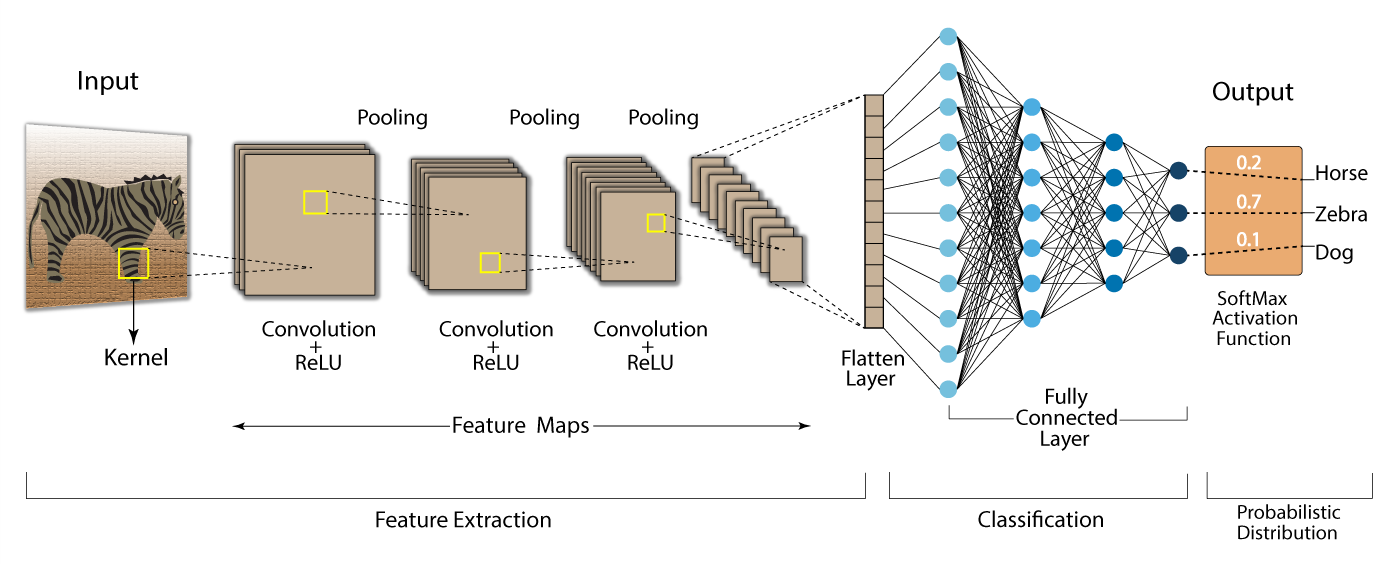
\includegraphics[width=\textwidth]{graphics/cnn_banner.png}
\end{figure}

\begin{figure}
    \centering
    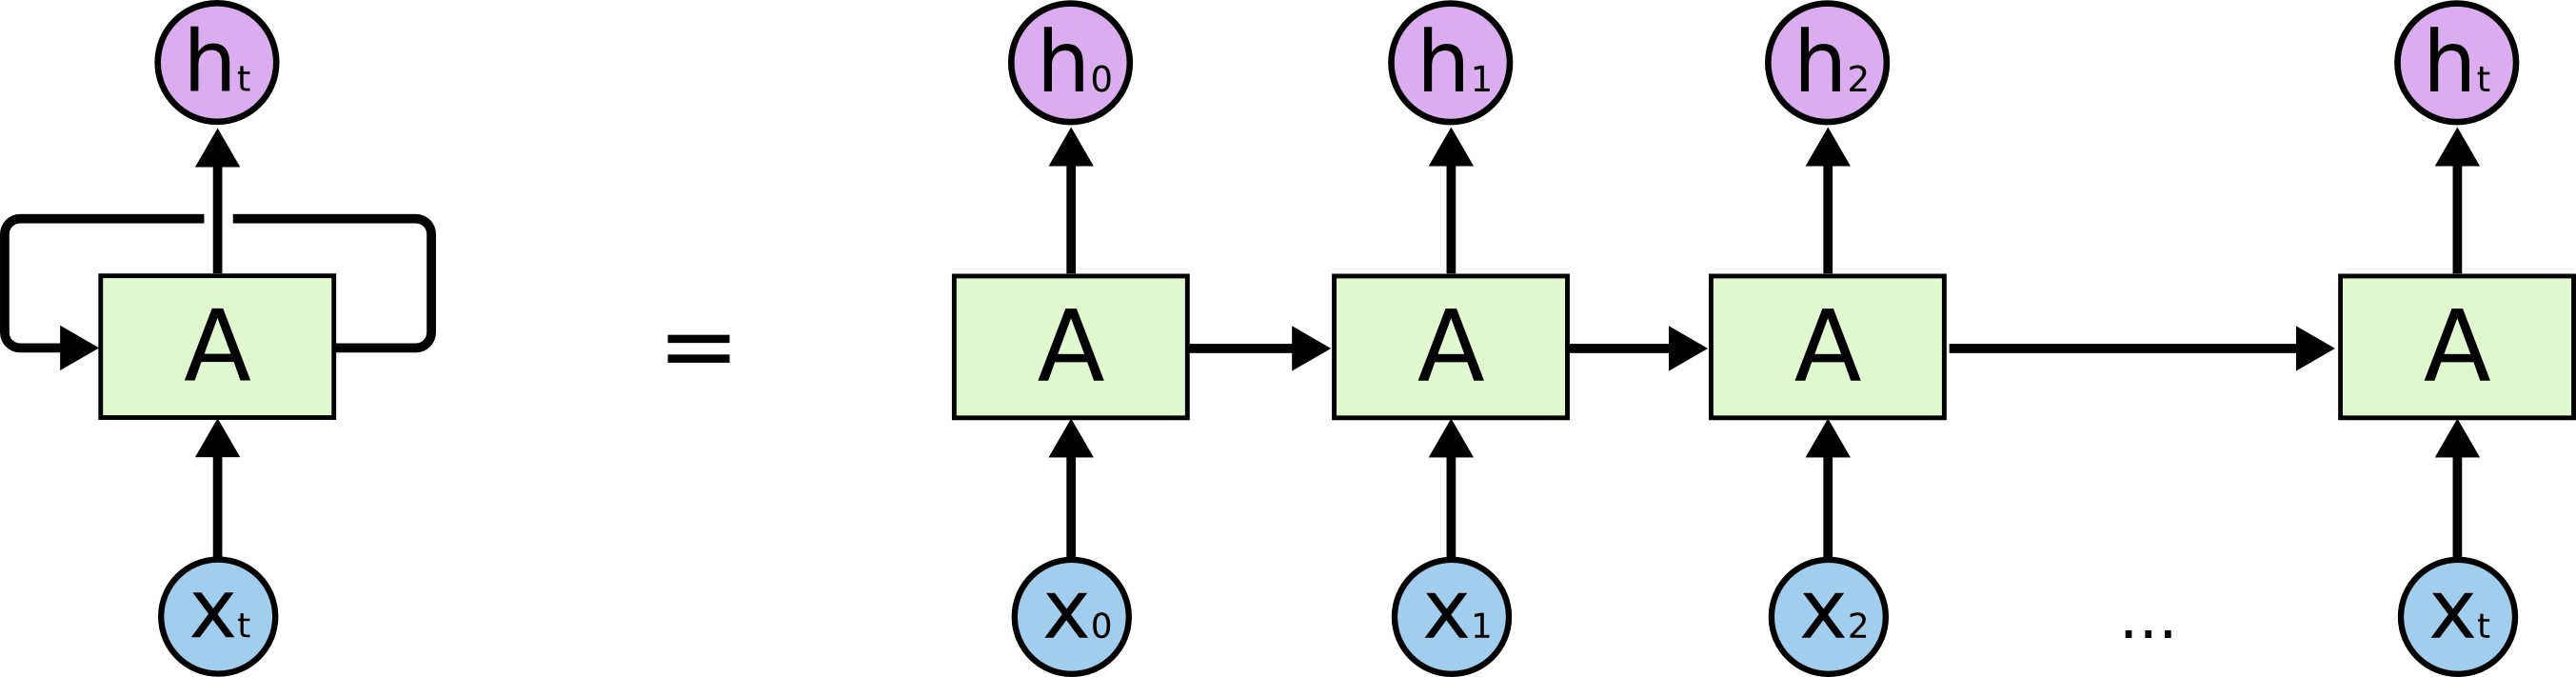
\includegraphics[width=0.7\textwidth]{graphics/RNN-unrolled.png}
\end{figure}

\newpage\subsection{Deep Learning in Space Exploration}

Disregarding the disagreements of whether space should be privatised or remain
only in the public sector, the uncertain economic returns of space exploration
are well known to be a key hindrance to progress in the field. Space
exploration is expensive, and this uncertainty of return is unattractive to
profit-seeking companies, leaving stakeholders far and few between. As a result,
the most successful results from \gls{DL} are rarely used in space exploration
due to neural networks not being human readable~\cite{esa_ai}. Interpretation of
neural networks have come a far way however, but require a deep understanding
of the problem domain for effective understanding of the way in which the
network is approaching its given task~\cite{Montavon2018, Sheu2020,
goh2021multimodal, molnar_2022}. The tasks most interpretable tend to be those
most relatable to the human mind, such as language
processing
\cite{belinkov-etal-2020-interpretability, DBLP:journals/corr/abs-2108-04840},
and visual pattern recognition \cite{DBLP:journals/corr/abs-1802-00121}.

\gls{DL} in space exploration has been a popular topic of research in recent
years, some examples of the learning tasks have followed directly from
promising methods in the following areas:

\begin{itemize}
    \item \textbf{Search for celestial patterns}: The detection of bodies in
          the solar system is dependent upon the size, distance from Earth, and
          albedo of the body in question. For asteroids, their albedos range
          from 0.03, for C-type asteroids, to 0.22 for S-type
          \cite{planetary_data}. These conditions result in a situation where
          expensive manual surveys are required to sift through large amounts of
          data in order to find potential detections. A recent trend in this
          area is the use of deep learning to find patterns in the data
          indicating the presence of these bodies. \glspl{CNN} have been used to
          detect asteroid trails in Hubble Space Telescope data
          \cite{parfeni2020detection}, and a two-stage detection-classification
          framework in the Asteroid Terrestial-impact Last Alert System (ATLAS)
          survey \cite{Chyba_Rabeendran_2021}. The reported accuracies on
          test data is promising, bringing humanity one step closer to
          autonomous detection of potentially hazardous (or opportunistic)
          asteroids. The applications of \gls{DL} have not been strictly limited
          to our Solar System, with exoplanet detection also showing promising
          results with limited datasets \cite{bird2020model}.

    \item \textbf{Uncooperative space objects}: A big threat to our future in
          space is the abundant presence of space debris trapped in orbit around
          Earth, which grows steadily as time passes, increasing the risk of a
          cascading series of collisions resulting in the Kessler Syndrome
          \cite{https://doi.org/10.1029/JA083iA06p02637}. This condition would
          have devastating consequences on our future presence in space. One of
          many required potential measures is the de-orbiting of larger space
          debris to avoid the risk of collision leading to smaller and less
          predictable debris. The use of deep learning to detect, classify, and
          track decommissioned spacecraft is a promising approach to the series
          of challenges in de-orbiting an uncooperative object. Space object
          classification \cite{doi:10.1177/0954410021996129, 8009786}, and
          pose estimation \cite{Afshar2020, Ren2020} are key learning tasks in this
          area of ongoing research, making extensive use of \glspl{CNN}.

    \item \textbf{Small body dynamics}: The mass distribution of asteroids are
           often heterogeneous and their shape far-off from spherical,
           spheroidal and ellipsoidal, presenting challenges when applying the
           trick of the trade in gravitational potential modelling, namely:
           spherical/spheroidal harmonics, and ellipsoidal harmonics. This
           was mentioned and discussed briefly in \autoref{sec:dynamic_modelling}
           \textcolor{(section on environment models)}. \gls{DL} shows promise
           in the area of asteroid dynamics, steadily progressing in the
           research community \cite{carruba2022machine}. One promising new
           alternative in gravitational potential modelling is the use of
           neural networks to model the mass density of a body, using neural
           density networks \cite{DBLP:journals/corr/abs-1802-00121}. The
           results of Izzo et al. in the latter task are particularly promising,
           as they have demonstrated that artificial neural networks can be used
           accurate geodetic models of highly irregular bodies given minimal
           prior information on the body. Their novel method is referred to as
           using a geodesyNet, which is a neural network that learns a
           three-dimensional, differentiable mapping of the body's density, that
           the authors refer to as a neural density
           field~\cite{IzzoGeodesyNet2021}. An interesting design choice in
           geodesyNet is the use of sine waves as activation functions, which
           had been notoriously difficult to train due to their periodic, and
           non monoticity (See \autoref{activation_fn}).

%    \item This novel approach is generic and can be used to
%           analyze geodetic properties of the body and even infer its body shape.
%           If provided with a body shape, the accuracy of the model improves
%           as well as reducing training times of the neural network.
%
%            \begin{equation}
%                \kappa = \frac{\sum^n_{i=1}\hat{y}_i{}y_i}{\sum^m_{i=1}y_i^2},
%            \end{equation}

%            which modifies the original \gls{MAE} (see \autoref{chap:ML}) loss
%            function to the following form:
%
%            \begin{equation}
%                \gls{J}_{\kappa\text{MAE}} = \frac{1}{\gls{ml:m}}\sum_{i=1}^{\gls{ml:m}}||{y}^{(i)}-\kappa{}\hat{y}^{(i)}||_1.
%                \label{eq:MAE}
%            \end{equation}

%            \begin{equation}

            \begin{figure}[H]
                \centering
                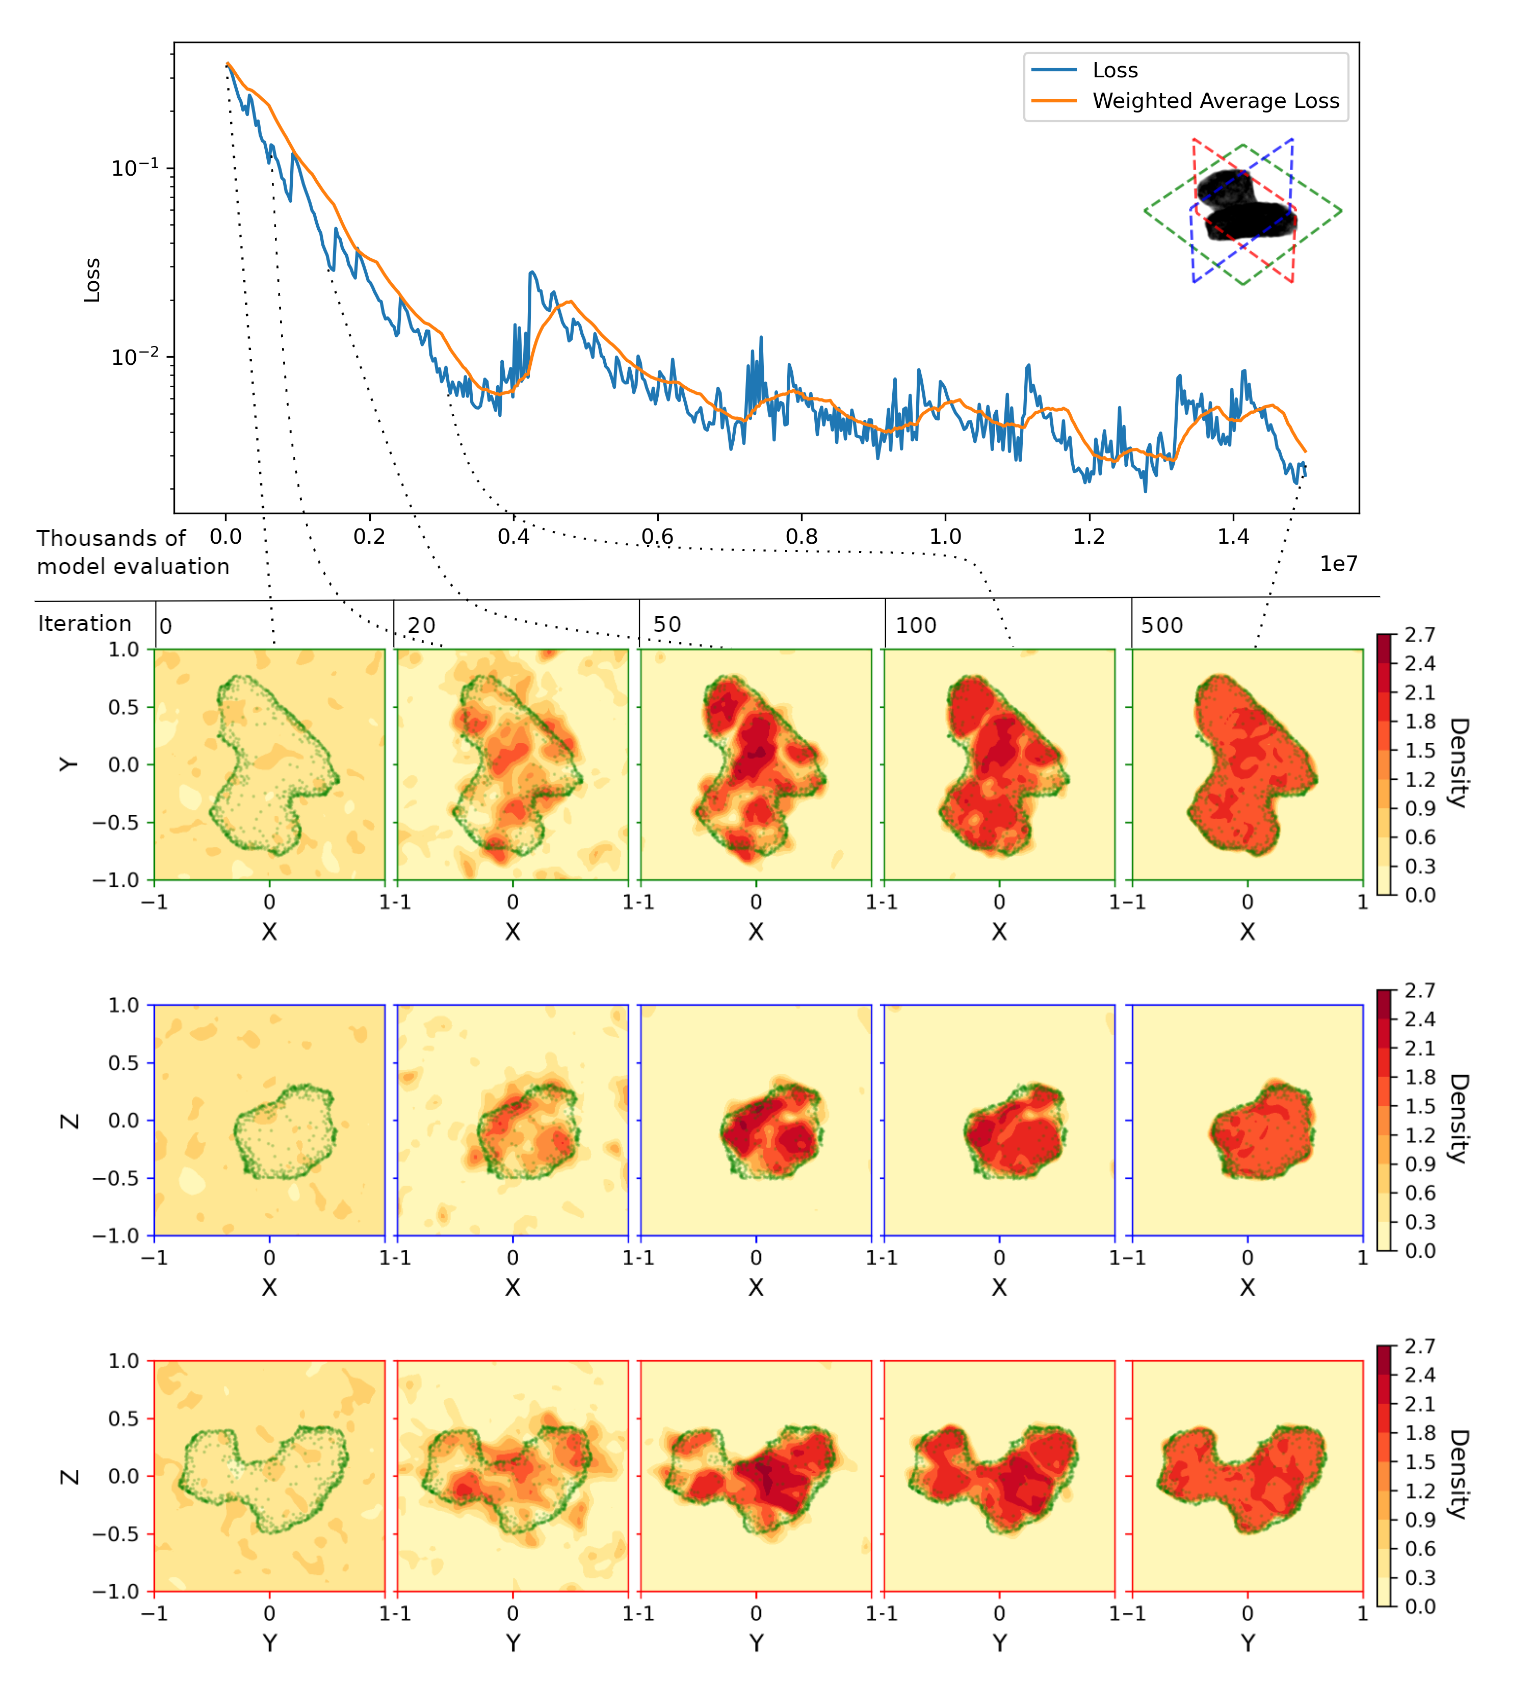
\includegraphics[width=0.8\linewidth]{graphics/geodesynet-example}
                \caption{GeodesyNet~\cite{IzzoGeodesyNet2021}}
                \label{fig:geodesy-net}
            \end{figure}


%    \item \cite{Takahashi2014}
%    \item and as a result of their shapes, they require two sets
%    of spherical harmonics expansions to describe their gravitational potential
%    outside of the body. One set is used to model the gravitational potential
%    outside the Brillouin (i.e., circumscribing) sphere of the body.

    \item \textbf{Low-thrust trajectory optimization}:

    \item \textbf{Trajectory sequence planning}
    \item \textbf{Spacecraft autonomous control}
\end{itemize}

been toward autonomy in docking
\cite{}, navigation, and environment modelling~\cite{IzzoGeodesyNet2021,
IzzoBennu2021}. The former two are tasks coupled within a joint
\gls{DL}-\gls{RL} framework, which are covered in \autoref{chap:RL}.

The authors use a modified \gls{MAE} loss
function to train the network, which allows the network to focus on learning the
deviation from a homogeneously filled volume $V$, and not concurrently the
absolute value of the body mass. This is achieved using the factor $\kappa$:





\cite{Kothari2020}